\documentclass[11pt, a5paper, openright]{book}

% This is a transcription done by Mairi Dulaney of Seattle, WA

% chktex-file 18

\usepackage{caption}
\usepackage[english]{babel}
\usepackage[T1]{fontenc}
\usepackage[]{geometry}
\usepackage{textcomp}
\usepackage{gensymb}
\usepackage{graphicx}
\graphicspath{{images/}}
\usepackage[utf8]{inputenc}
\usepackage{makeidx}
\usepackage[round,sort,comma]{natbib}
\usepackage{rotating}
\usepackage{titlesec}

\usepackage[activate={true,nocompatibility},final,
  tracking=true,kerning=true,factor=1100,stretch=10,shrink=10]{microtype}

\geometry{a5paper}
\nonfrenchspacing

\widowpenalty10000
\clubpenalty10000

\titleformat{\part}[display]{\centering\normalfont\Huge\bfseries}{}{0pt}{}

\titleformat{\chapter}[display]
{\bfseries\Large}
{\centering
  \textsc{Chapter} \thechapter.}
{0.5ex}
{
  \vspace{1ex}
  \centering
  \scshape
}
[\vspace{-1ex}]

\titleformat{\section}[display]{\centering\bf}{\enspace}{0em}{}

%\overfullrule=2cm

\renewcommand{\thefootnote}{\fnsymbol{footnote}}


% Some macros to make indexit easier
\newcommand{\barge}[1]{\textit{#1}\index{#1,~barge}}
\newcommand{\steamer}[1]{\textit{#1}\index{#1,~steamer}}
\newcommand{\steamerco}[1]{#1\index{#1}}
\newcommand{\gastug}[1]{\textit{#1}\index{#1,~gas tug}}

\makeindex


\begin{document}

\renewcommand{\thechapter}{\Roman{chapter}}
\title{Riverboating in Lower Carolina}
\author{F. Roy Johnson}
\date{1977}
\bibliographystyle{alpha}
\maketitle

\index{Cape Fear Steamboat Company|see {Cape Fear Line}} %chktex 24
\index{Claremont|see {\textit{North River}}} % chktex 24
\index{C.~W.~Lyon|see {\textit{A.~P.~Hurt}}} % chktex 24
\index{Henrietta Steamship Company|see {Henrietta Steamboat Company}} % chktex 24
\index{Lutterloh \& Company|see {Lutterloh Line}} % chktex 24
\index{Oast|see {\textit{Pioneer}}} % chktex 24
\index{Bostic|see {\textit{Brook}}} % chktex 24


\part{I}

\chapter{By Paddle, Ore, and Pole}

\section{Early Boats of Burden}

\textsc{Although} the dugout canoe, or log boat, has disappeared from
the rivers, creeks, and other waters of North Carolina's southeastern
counties, the watersheds of the Cape Fear, Black, and Northeast
rivers, it must be remembered as the common and more important vehicle
of travel and commerce of the early settlers of the region.  And to a
diminishing extent this versatile vehicle continued in common service
far into the nineteenth century.  As late as the 1950's a few
serviceable old moss cloaked log boats reposed in the South River
wilds of Bladen and Sampson counties and at remote landings of the
upper Waccamaw River in Columbus County.\par

The numerous waterways of the southeastern area --- the sounds, the
rivers, and the creeks --- were well suited for small boats.  These
avenues grew into the great channels of commerce and retained their
commanding position for nearly two centuries, until the railroads
became common and transportation needs moved westward.\par

Although much of the early travel was overland by horseback and by
foot on trails little better than Indian paths, virtually all the
commerce was by water.  However, by the Revolution, overland traffic
had increased; for the industrious settlers had built roads,
constructed causeways across swamps, bridged streams, and established
ferries.  This lessened little the water freightage.  And up and down
the waterways there plied a great variety of craft loaded with
commodities.\par

Plantations, trading places, villages, and towns sprang up along the
streams; and the growth of the towns was determined to a large extent
by the volume of this commerce.  Chief of the towns were Fayetteville
at the head of navigation on the Cape Fear River, which funneled goods
down stream from the back country and received imported commodities,
and Wilmington, which exported and imported goods for the watersheds
of the Cape Fear River and her tributaries.\par

Not so fortunate was the town of Lisbon at the head of the Black River
in Sampson County.  Its merchants prospered and the town grew and
flourished on pole boat traffic.  But after steamboats came it went
neglected because of the river's shallows; and it dried up completely
when bypassed by the railroads.\par

\section{The Canoe and Periauger}

The canoe's larger companion, the periauger, was a boat of burden
which served in the early commerce of the southeastern counties.  And
as the volume of commerce increased it was followed by the larger flat
boat, or pole boat.\par

Writing in 1737, a time when settlers were pouring into the
southeastern area, Dr.\ John Brickell told of the building and use of
the canoe and the periauger.  The canoe, eh said, was made out of one
piece of timber and commonly of cypress, the durable giant of the
coastal swamp forests.  A log of proper thickness and length was cut
from the felled tree, and craftsmen shaped the log like a boat and
then hollowed it out.  Sometimes the boat was made wider by splitting
it down the middle and installing boards in its bottom; and this boat
was called the periauger.  Then the canoe or periauger was fitted with
masts for sailing or oars and paddles, ``according to \ldots size and
bigness.''\par

Some of the larger of these craft were ``capable of carrying forty or
fifty Barrels of Pitch and Tar.''  The planters also found the
periauger useful as ferries and for transporting goods from one
plantation to another.  The design of this great log boat made it so
efficient that ``no Vessel of the same Burthen made after the European
manner'' could outsail one.\citep[260-261]{brickellj}\par

William Robinson, a Sampson County planter who lived at the Delta on
the Black River about sixty miles from Wilmington by water, was using
a large cypress log boat in regular commerce with that seaport town in
the late eighteenth century.  He manned her with six black oarsmen.
And late in the nineteenth century William's great-grandson Scott
Robinson was running a turpentine distillery at the Delta and
freighting naval stores to Wilmington on a fifty foot by twelve foot
flat poled by four blacks.  \citep{shawg}\par

The canoe was made in many sizes.  The smaller might carry no more
than two or three men while the larger could carry two or three
horses.  They seem to have continued quite numerous throughout the
eighteenth century.  During the spring of 1762 a group of Moravians
proceeding up the Cape Fear River watched their boats by night for
fear of Negroes who ``go about in small canoes, stealing where they
can.'' \citep[I,~261]{friesal}.  And in 1775 Janet Schaw, a Scotch
woman sojourning in North Carolina, saw more than one hundred people of
the lower class in canoes come to a funeral on the Northeast
River.\citep[171]{schawj}\par

The larger boats used sails to great advantage, except on narrow and
croked streams where oars and poles were needed.  Tides favored all
kinds of craft upon the lower rivers, and freshet waters often aided
navigation upon their headwaters.\par

\section{Eighteenth Century Row Boats}

Late in the eighteenth century large \textit{row boats} were the
carriers of produce on the Cape Fear River between Cross Creek, near
present Fayetteville, and the Wilmington area \citep[280-281]{schawj}.
The planter near Wilmington manned such boats with slaves.  For travel
one such planter had ``a very fine boat with an awning to prevent the
heat and six stout Negroes in neat uniforms to row her down, which with
the assistance of the tide was performed in a very short time''
\citep[177]{schawj}.\par

As the volume of commerce increased, so did the size of the boats.
This led to the construction of the flat boat, or \textit{flat}, so
called because of its flat bottom and squared sides, which was built
of boards.  Being of shallow draught it could be used on small
streams.\par

Navigation of the streams often was beset with problems.  Hugh
Meredith, who about 1730 had come to North Carolina from Pennsylvania
to settle, wrote that the channel of the Northeast Cape Fear River was
impeded by the ``multitude of Logs that lie in it, part of them fast in
the Sand, with great Snags or Limbs, and sometimes either End the
Middle quite above, or but little beneath the Surface; and in some
places we saw whole Heaps jumbled together, almost from Side to Side,
and so firm that they are immovable, being sound, heavy, fast, and
deep in the Sand.'' (Meredith, Hugh, 21-22).\par % chktex 8

Soon after the Revolution there was a burst of enthusiasm for
improvement of waterways for navigation.  Some progress was made in
making passable the channels of the main streams.  And by the opening
of the nineteenth century virtually every little stream was cleared of
obstructions so as to accomodate small boats and flats, giving many
farmers located off the large streams access to water
transportation.\par

\section{The Pole Boat}

South (Black) River, a tributary of the Black River, which rises in
Harnett County, was an important avenue of commerce for farmers of
eastern Cumberland County.  They ran their rafts and pole boats upon
it until late in the nineteenth century when railroads provided an
alternate means of transportation.\par

Caleb C. Bullard, born in 1859 in Beaverdam Township, recalled that
naval stores were carried down from this area to Wilmington on flat
boats.  John A. Oates in his \textit{The Story of Fayetteville} quotes
Bullard as saying, ``There was no trouble in getting down the river,
except to keep the flat boat guided; there was no steam power on South
River.  It took usually about four days for the trip down and six days
for the trip back, about 100 miles each way.  In Wilmington, they
would secure, usually, a tug boat to bring them to the mouth of South
River and from there up they would use poles twenty feet long or more,
to push the flat boat on up the river.  They would have six or eight
men to do this.''\par

Naval stores were the chief source of income for the Cumberland
farmers until some time after the Civil War when they began to raise
cotton.  In the depressed economy they found little inducement to grow
more than enough food to feed their families and livestock
\citep[432]{oatesja}.\par

\section{The Large Flat of Tidewater}

In tidewater no other power than the tide was needed to move the large
flat.  It was tied up against the tide, and when the tide turned it
floated like a raft with it.  Large flats, some carrying as much as 100
to 200 barrels of turpentine, tar, and pitch, were in use upon the
lower Cape Fear before the Revolution \citep[184-185]{schawj}, but
smaller craft were common above tidewater until the coming of the
steamboat which could tow them upstream against the current.\par

Some idea of flat boat sizes early in the nineteenth century may be
obtained from an advertisement in the November 21, 1816
\textit{Fayetteville American}.  An advertiser was seeking to let a
contract for construction of four flat boats, two 48 feet by ten feet
and two 30 feet by six feet.  They were to be made of heavy timber and
sides banded with strap iron \citep[11-21-16]{fa}.\par

Midway through the nineteenth century tide powered flats were carrying
300 to 500 barrels of turpentine or an equal amount of other
cargo.\footnote{The Wilmington Journal of 1851, under ``Marine
  Intelligence'', provides a record of pole boat activity.}  For
example, flat boat
\textit{J.~L.~Cassidy}\index{J.~L.~Cassidy, flatboat} from Lyons
Landing on the lower Black River arrived in Wilmington on April 11,
1851 with 326 barrels of rosin, 64 barrels of tar, and 64 barrels
of turpentine.  By comparison, on January 31 the flat boat
\textit{Sopha}, with Man William in charge, from Beatty's Bridge on
the Black River 50 miles above Wilmington and above tidewater, arrived
with 38 bales of hay, five bales of fodder, and four sheafs of oats.
It's cargo was comparable to about ten barrels of turpentine.\par

Meanwhile, the large tide powered flat boat was hauling much of the
cargo on the lower Cape Fear, Black, and Northeast rivers.  White
Hall, on the Cape Fear about 18 miles below present Elizabethtown and
54 miles above Wilmington became an important receiving and trading
center.  With some assistance from poles the great flats were able to
make their way this far up with no great difficulty.  Those going
higher up mostly were towed by steamboats.  Some of these, especially
those owned by the steamboat companies, were towed back down stream;
and these were called \textit{tow boats}.\par

Often the large flat boat was given a name which honored its owner or
some other person and put in charge of a trusted slave.  In 1851 one
finds Man Dick in charge of \textit{Uncle Sam}; Man Sandy, the
\textit{David Lewis}, Man Bob, the \textit{Stevenson}; Man Wilson, the
\textit{General Taylor}; Man Jack, the \textit{Dried Apple}; Man
Daniel, the \textit{James Ellis}; Man Dick, the
\textit{J.~L.~Cassidy}.  Other big flats were the \textit{David Reed},
the \textit{Jackson}, the \textit{General Cass}, \textit{Macmillan's Boat},
and \textit{Robinson's Boat}.\par

\section{The Steam Flat}

The steam flat followed the pole and row boat and small flat into the
narrow and shallow headwaters of the Black and Northeast rivers and
large creeks to compete with rafts in bringing down naval stores from
the developing country.  Although some of the early steamboats on the
Cape Fear River were little more than steam-powered paddle-wheel
flats, the steam flat as a distinctively different kind of craft did
not appear until after the Civil War when the entire southeastern area
of North Carolina was faced with the need for economical
transportation.\par

In 1886 ten of these vehicles of burden were transporting naval stores
and other commodities from the back country of Bladen, Brunswick,
Pender, Sampson, and Onslow counties to Wilmington.  Two of these were
operated on the Great Coharie, a shallow tributary of the Black River
up to 100 miles from Wilmington.  \citep[8-13-86]{ws}\par


\chapter{The Raft Runners}

\textit{\textsc{When} the Lord was making the world He had a lot of
  river left over, so he doubled it up and made it into the South
  (Black) River.  Thus, said the old folks, is how this stream came to
  be so crooked.}  \citep{shawg}\par

South River also is narrow.\par

Yet the small white farmers of Bladen, Sampson, and Cumberland
counties floated down their logs and barrels of naval stores to Black
River where they were formed into rafts and carried on to market in
Wilmington.\par

Both these and other Sampson County farmers who came down Six Runs and
the Coharies to the Black River were a hard working and hardy set of
people.  They came in winter and early spring when the streams were in
freshet and when the weather was cold and nasty.\par

To the people of the lower river they were strangers from a seemingly
vast and mysterious country.\par

Although tough and rugged they were strangers with some pleasant tune
on their lips except when fighting the wiles of the river, the
swirling currents of sharp bends, and the eddies braking and twisting
their train of logs.\par

These were strangers who were ever ready to hail a ``Hello there!'' to
any person who would return their greeting.\par

Some of the raft runners, several days from their upriver homes, seemd
a bit lonely.  While sitting beside their campfire or riding the river
current they dismissed a part of their solitude and at the same time
awakened lonely countrysides with hooting, hollering, singing, and
whistling.  The ddep river swamps amplified and echoed these sounds,
and at times they could be heard for many miles.  So those dwellers
beside the main dusty road, which followed near by the river, and
others afar might hear musical strains that belonged to earlier times
when raft runners of earlier generations passed this same way.\par

They rode rafts of many kinds.  From colonial times on past the Civil
War they carried to market choice timbers for masts and spars for
sailing ships, squared logs, or ton timber, for sawmills, and naval
stores, like turpentine, rosin, and tar in trains of barrels.  After
ascendance of the railroads cross ties were stacked, clamped, and
formed into sections like log bateaux to form rafts; these were
floated to the rail heads in Wilmington.  Log rafts upon large waters
might contain as many as five hundred logs with bateau after bateau
following in tandem.\par

\section[Stream Clearance Scheme]{A Stream Clearance Scheme}

By the opening of the twentieth century, rafting on the Black River
had gone on so long that it had become an institution.  Upon her
tributaries a hundred years earlier, people were questing after an
unobstructed water avenue to market.  Announcement of a lottery was
made in the April 5, 1811, \textit{Cape Fear Recorder}; and it stated
that the ``scheme was for the purpose of clearing and making navigable
for rafts and boats the main branch of the Six Runs in Sampson County,
from Kerby's Landing to Fryer's Bridge, so called.''
\citep[4-5-11]{cfr}.  Soon after 1900 and following heavy rains a
Harrells farmer floated cross ties down nearby Bulltail Swamp to Black
River and on to market \citep[]{melvinew}.  Narrow rafts, six or eight
logs wide, could be brought down South River, a long and crooked Black
River tributary, from the vicinity of Dunn in Harnett County
\citep[]{johnsonlg}.\par

Large Numbers of rafts came down the Black River and other streams of
North Carolina's southeast.  The December 17, 1852 Wilmington
\textit{Journal} stated, ``about 100 rafts of timber changed hands''
during the previous week.  Then on December 24 following it explained:
``The water courses have been high for some time, and produce such as
timber, Turpentine, Lumber \&c, usually dependent upon the state of
the rivers, has been coming in abundantly lately.''\par

\section[An Adventure]{An Adeventure of an Eight-Year-Old Boy}

Sometimes the farmers brought along their young sons for the adventure
and to teach them the ways of the river.  A vivid account of raft
running during winter has been given by Campbell Johnson, a Bladen
County boy who at the age of eight or ten years made a trip by raft to
Wilmington, a city of wonders for country children.\par

The loud cry of a steamboat whistle came thundering down the river,
from around a far-away bend of the the yellow water Cape Fear River.
It cried again and again warning any craft it might be meeting.  It
was a welcome and a thrilling call for the boy; for this was the first
familiar thing he had experienced on the new and strange lower river.
He had been hearing the same steam whistle as far back as he could
remember, for it frequently broke the monotony of the quiet
countryside near his home in Rowan community, Bladen County, about
forty miles upstream as the boat plied the Black River, a Cape Fear
tributary.\par

``The \textit{Liz}!'' the boy cried as he bounded from beneath an
inverted log boat sheltering him from the cold drizzling rain.\par

He was on a log raft basking before a roaring log fire.  His father
and two helpers had tied up their raft at Long Reach on the Cape Fear
to await the change of the tide which would give them a free ride
several miles more to the sawmill in Wilmington.  The \textit{Lisbon},
which some Black River folks called \textit{Old Liz}, was Captain
D.~J.\ Black's\index{Black, Captain D.~Jasper} river steamer.  She was
coming down from Clear Run, twelve miles below the town of Lisbon and
the confluence of Six Runs and Great Coharie.  Captain Black lived at
Point Caswell, and he and \textit{Old Liz} paddled up and down both
the Black and Cape Fear rivers picking up and delivering freight and
carrying a few passengers.\par

Soon after the \textit{Lisbon's} whistle blasts the thumping and
pounding of her steam engine floated down the river, and she came
around the far-away bend.  The boy fastened his eyes upriver like
folks waiting at river landings upon the approach of a steamer.  It
was practically no time before the \textit{Lisbon} drew near.  White
spray frothed about her low bow which seemed to plow a furrow in the
river like a farmer in his field.  The boat slowed, and as her
whistled signaled a greeting ``boop, boop, boop'' the captain waved
from his pilot house to the men and the boy on the raft.\par

\section{Hard Life on the River}

Although the hardy men along the rivers refused to let foul weather
hinder them in their raft running, they often talked about the
discomfort and hardships they suffered.\par

Except for a few rude shelters they were exposed to the weather.  Soon
after 1900, for example, Frank Sessoms, a storekeeper at Long View on
the Black River, provided some comfort for the raft men coming down
from Sampson and Cumberland Counties.  He had an old shanty for them
to camp out in when the weather was bad.  \citep[]{rawlsgw}\par

But, the Bladen County rafters had no shelter once they left
Sparkleberry near Mill Creek on the Black River before daybreak the
morning of the previous day.  At Sparkleberry where the river widens
the narrow long rafts which had run the \textit{Narrows} were widened.
The big raft now was actually a train of bateaux, a bateau being a
section of a dozen or more logs fastened side by side at each end with
batten poles.  In 1900 hickory pegs were driven into holes bored
through the batten poles into the logs.  A few years later sixty penny
size spikes replaced the wooden pegs.\par

Already, the rain had begun to come down in a cold drizzle.  The men
prepared for a hard trip.  They placed boards side by side across the
logs of the front bateau.  They covered the boards with a layer of
dirt, and this enabled them to build a fire.  They piled nearby a tall
stack of fire wood cut from small trees.\par

Before the ropes holding the raft fore and aft were untied and the
raft set upon its one to two mile-an-hour drift the fire was roaring.
But the rain grew heavier, and the boy stood near the fire as moisture
steamed from his wet clothes.  One of the three men steered the course
of the raft with a long home-made oar which extended ahead of the
front bateau.  A second man worked from section to section on the rear
bateaux making certain they ran clear of obstructions.  The third man
took his turn before the fire and was ready to help when and where
needed.\par

The wooden \textit{cracker box}\footnote{Crackers carried by country
  storekeepers came packed in wooden boxes.  The empty boxes found
  many uses; one was for packing food for picnics and as in this
  instance a trip of several days.}, filled with food for a trip of
three or four days, stood out in the rain.  The women folks back home
had packed it with home-made cookies known as \textit{tea cakes}, fat
crusty flour biscuits and boiled meats.  In addition, there were meal
for fresh corn bread, eggs, lard, and a pan for frying, fishing lines
and fat meat to entice catfish during hours when the raft was tied up
against the inflowing tide.\par

The raft reached Racoon Island near the mouth of the Black River the
two tides it rode the first day.  Here it was tied up for the night.
The men seemed tired from a long day's work.  After eating supper they
``wrapped quilts around their heads'' and lay around the open fire.
They went to sleep with apparent ease even though the rain streamed
down cold.\par

By the following afternoon the raft had ridden the tide to Long Reach
where it was tied up to await the next outflowing tide.  The bateaux
lay end to end beside the tall grass of the marshlands where only a
few years earlier there had been rich rice fields.  Sand banks rose up
high on the opposite side of the river; they were known as
\textit{Mount Misery}.  Except for scattered scrub oaks and pines the
place seemed desert-like.  Perhaps its massive desolation made it one
of the more impressive landmarks witnessed by those who traveled the
lower Cape Fear River.\par

Beyond the march grass where the land rose to higher ground, smoke
lazed from the mud and stick chimney of a small cabin and drifted in a
foggy layer towards the ground.  Openings between the logs in the
cabin's walls had been daubed with clay.  The cabin looked old and
time-worn like the old black man and his woman who made it their home;
but the cabin was warm inside, and the boy enjoyed the hospitality of
the plain hearth.\par

The old man tilled a small plot of farm land which rose above the
marshes; and his chickens and hogs enjoyed open range.\par

His hogs were of unusual appearance to the boy who was accustomed to
the wild razorbacks of the swamps and great woods and the red and
black spotted ones back home in pens and pastures.  These hogs were
Blue guineas, the old man said.  The boy begged his father to buy him
a small gilt.  The father thought and then said, ``Maybe we can get
her home'' and paid the two dollars the old man asked.\par

Later, at Wilmington, Captain Black\index{Black, Captain D.~Jasper} was
told of the purchase, and he said he could take the hog on his next
trip upriver.  Such cargo was not unusual for Black River steamboats.
Their masters were accustomed to hauling almost anything the farmers
wanted to ship, including chickens, eggs, hogs, sheep, and cattle.\par

Early the next morning the three raft runners and the boy caught the
incoming tide and sent their twenty-foot-long log boat skimming the
solitary waters for home.  Early that night they arrived at David's
Landing, one mile along the public road from home, having paddled
forty-eight miles.\par

The following afternoon the \textit{Lisbon} arrived with \textit{Liz}.
The boy had named the gilt in honor of
Captain Black's\index{Black, Captain D.~Jasper} boat.  \citep{johnsonwc}\par

\section{The Prized Piano}

Sometimes Sampson County farmers above the head of navigation for
Black River steamboats would carry their farm produce to market on
their squared timber or log rafts.  The produce, chiefly corn, cotton,
hay, and bacon was piled atop a decking of loose boards, which too
were sold with the raft.\par

This had been the custom of Haywood J.\ Peterson, a Sampson County
farmer who lived near Clinton.  At the age of sixty-two in 1891
Peterson decided to move to Point Caswell on the lower Black River and
go into semi-retirement.  He sold his farm, loaded his household
furniture on a raft, and this rode a freshet down the Great Coharie
and the Black River to its destination.  But Peterson's daughter,
Hyancith, who was to become the wife of Captain
D.~J.\ Black\index{Black, Captain D.~Jasper}, would not trust her prized
piano on the raft.  It was too dangerous, she insisted; so the piano
was carried overland by horse and wagon.  It was delivered safely,
although a bit shaken by the rough roads, to the Point Caswell Hotel
where the family would live until a dwelling could be built.\par

A lively freshet carried the raft down swiftly.  The water was so high
that in places it streamed over the river banks into the bordering
swamps.  The raft runners fought to avoid being drawn into the forests
and demolished.  At one point they lost control and the current
carried their raft beneath an overhanging limb which swept a part of
the furnishings into the river.  Those which floated were picked up
and saved; but the sinkables, such as the family's treasured
silverware, were lost.\par

Hyancith treasured her piano until her death in 1976.\\
\citep{shumpertsb}.\par

\section{The Snow Train}

Once while recounting the rigors of raft running, one tough lumberjack
told of a trip down the Waccamaw River.  He was drifting a raft of
about 300 logs by himself, and a blinding snowstorm forced him to tie
up before nightfall.\par

He went ashore, gathered a quantity of fire wood, constructed a
lean-to shelter and made a bed of pin straw and Spanish moss.\par

He built a large fire in front of the shelter, ate his supper and
slept warmly while the wind howled and the snow came down.  By morning
the snow was about two feet deep, and his shelter was much like an
igloo.  His raft, decked in white, contrasted sharply with the black
water in the river.\par

The storm had mostly blown over, and he resumed his journey with the
current.  Two days later he arrived at the mill where no snow had
fallen.  He became the center of attention as a crowd of people lined
the river bank to admire his long procession of snow clad logs.
\citep{stevensjg}.\par

\makeatletter\@openrightfalse%

\part{II}

\begin{figure}[htb]
\centering
  \begin{turn}{90}
      \begin{minipage}{5.8in}
        \centering
        
\includegraphics[scale=.18]{ballous_pictorial_24_feb_1855_pp_121}\newline
        \textsc{Market Street, Wilmington, N.~C.}\newline---Ballou's Pictorial Feb.~1855
      \end{minipage}
    \end{turn}
\end{figure}

\chapter{The First Steamboats}
\@openrighttrue\makeatother

\section{The Monopolies}

\textsc{The} year 1818 marked the beginning of steamboat navigation in
eastern North Carolina when two paddle wheel steamers were put into
service on the Cape Fear River and a third one on the Neuse.\par

The Cape Fear steamers where the \steamer{Henrietta}, which was built
at Fayetteville by James Seawell\index{Seawell, James} to run between
that point and Wilmington, and the \steamer{Prometheus}, which was
built at Beaufort by Captain Otway Burns\index{Burns, Captain Otway},
famed as master of the privateer
\textit{Snap~Dragon}\index{Snap~Dragon,~privateer}, for a stock
company, which may have been the Cape Fear Navigation Company.  The
\steamer{Prometheus} was put in service on the lower river between
Wilmington and Smithville, now Southport.\par

The Neuse steamer was the \steamer{Norfolk}, built out of state and
purchased by the \steamerco{New Bern Steamboat Company}.  Thomas H.
Sloan in his \textit{Inland Steam Navigation in North Carolina 1818-1900}, % chktex 8
citing the New Bern \textit{Centinel} of April 11, 1818, states that
the \steamer{Norfolk} arrived in New Bern April 10 and thus became the
first steamer to go into service in the state.  Twenty days later, on
April 30, according to the May 9 Centinel, the \steamer{Henrietta} was
launched on the Cape Fear; and the July 23 \textit{National Intelligencer}
of Washington D.~C., tells of her first trip to Wilmington.  The June
13 \textit{Intelligencer} had stated that the \steamer{Prometheus} had
arrived at Wilmington and that within a few days she would probably
commence running from that place to Smithville.\par

These reports seem to establish the \steamer{Norfolk} as the first
steamboat service in North Carolina and the \steamer{Henrietta} as the
first steamship built in this state.\par

However, unsuccessful steps to introduce steamboat service had been
taken several years earlier.  Robert Fulton\index{Fulton,~Robert} had
made his first successful voyage on the Hudson River with his
steamboat \steamer{North~River}, otherwise known as
\textit{Claremont}\index{North~River,~steamer}, eleven years
before the \steamer{Henrietta} and the \steamer{Prometheus} began
service on the Cape Fear.\par

A proposal to bring steamboat service to North Carolina was made by
John Stevens, of Hoboken, New Jersey, in 1812 when he presented a
memorial to the State legislature.\par

In response an act was passed ``for the encouragement of Steam Boats
on the waters of this State.''  By this act, Stevens and his
associates were given a twenty year monopoly for steamboat operation.
But, the act provided that Stevens must have a boat in operation
within two years for the monopoly to continue on force.
\citep[12]{sloanth}.\par

Stevens' monopoly was met with several protests, one being made by
Fulton.  Even though his monopoly was declared valid by the
legislature, Stevens failed to establish steamboat service as
provided.  It lapsed in 1814, and the legislature refused to grant his
request for renewal even though he explained that he had built the
steamer \textit{Phoenix} for this service and the British blockade of
the coast during the War of 1812 had forced her to remain in the
harbor at Hoboken.  \citep[1-3]{turlingtonsw}.\par

The protests and ensuing debates in the legislature for the improved
transportation that steamboats would provide aroused widespread
interest in steam navigation.  One of the main obstacles was the poor
condition of the rivers.  The presence of logs and snags made
navigation extremely difficult and hazardous.  However, steps were
taken to remedy the difficulties.  The Cape Fear Navigation Company
had its original stock supplemented with \$50,000 in private
subscriptions.  Work began on the river before august 1816, and
Archibald Murphey stated in 1819 that, ``the river is navigable for
Steam-Boats to Fayetteville, and may be probably rendered navigable
for small Steam-Boats to Haywood.''  \citep[7, 11]{turlingtonsw}.\par

By 1838 the Cape Fear Navigation Company had removed 1159 trees, logs,
and stumps from the river.  Wing dams had been built, and navigation
on the Cape Fear was considered ``better, safer, less liable to
interruption from low water, and by far cheaper than any river south
of the Potomac, of the same size and extent.''  By this time the
steamboat \steamer{Henrietta} had run the river for twenty years
without being snagged or meeting with any serious accident.
\citep[12, 13]{turlingtonsw}.\par

After turning down a petition in 1817 by Joseph
Seawell\index{Seawell, Joseph} of Fayetteville, the General Assembly
of the following year granted him a monopoly for steam navigation
between Wilmington and Fayetteville.  His petition stated that he had
a boat under construction.\par

The bill gave Seawell\index{Seawell, Joseph} and his associates ``the
sole and exclusive right and privilege of using, employing, and
navigating all and every species or kinds of boats propelled by the
force of steam on the waters of the Cape Fear river between the towns
of Fayetteville and Wilmington for and during the full term of seven
years from and after the passage of this act.''
\citep[22]{turlingtonsw}\citep[13]{sloanth}.\par

Launching of the \steamer{Henrietta} at Fayetteville and arrival of
the \steamer{Prometheus} at Wilmington were met with great
enthusiasm.\par

\section{The \textit{Prometheus}}

The \steamer{Prometheus} was brought down from Beaufort by Captain
Thomas N.~Gautier\index{Gauitier, Captain Thomas N.}, a worthy old sea
captain.  Colonel J.~G.~Burr told the story of her arrival to James
Sprunt who gives it in his
\textit{The Chronicles of the Cape Fear River}.
\citep[139]{spruntj1916}.\par

``Expectations were on tiptoe after the departure of the captain; a
feverish excitement existed in the community, which daily increased,
as nothing was heard from him for a time, owing to the irregularity of
the mails; but early one morning this anxiety broke into the wildest
enthusiasm when it was announced that the \steamer{Prometheus} was in
the river and had turned the Dram Tree.  Bells were rung, cannon
fired, and the entire population, without regard to age, sex, or
color, thronged the wharves to welcome her arrival.  The tide was at
the ebb, and the struggle between the advancing steamer and the fierce
current was a desperate one; for she panted fearfully, as though
wind-blown and exhausted.  She could be seen in the distance,
enveloped in smoke, and the scream of her high-pressure engine
reverberated through the woods, while she slowly but surely crept
along.  As she neared Market Dock, \ldots the captain called through
his speaking trumpet to the engineer below: `give it to her, Snyder';
and while Snyder gave her all the steam she could bear, the laboring
\steamer{Prometheus} snorted by, amid the cheers of the excited
multitude.''  \citep[139]{spruntj1916}.\par

The \steamer{Prometheus} was in operation in 1819 when President James
Monroe and his party were hospitably entertained in Wilmington.  On
his departure the President was taken to Smithville on the new
steamboat.  \citep[4-27-1819]{ni}\par.

But the low-powered \steamer{Prometheus} seems to have been less than a
financial success; she was abandoned in 1825, only seven years after
her launching.  \citep[19]{sloanth}.\par

\section{The \textit{Henrietta}}

But the story of the \steamer{Henrietta} was quite a different one
from that of the \steamer{Prometheus}.  As a trail blazer for other
pioneer steamboats on the Cape Fear River her long life and financial
success was remarkable.\par

She was built by James Seawell\index{Seawell, James} in 1817-18, on % chktex 8
his plantation on the east side of the Cape Fear River three miles
above Campbellton, now Fayetteville.  Seawell\index{Seawell, James}
named the boat for his daughter Henrietta.  A large concourse of
people attended her launching on April 30, 1818.  Then she was put
under command of Captain Charles Taws\index{Taws, Captain Charles}.
\citep[429]{oatesja}.\par

Many flat, or pole, boats had been constructed in the Campbellton
area, and the \steamer{Henrietta}'s sturdy hull must have profited
from the skill of local ship carpenters.  \citep[428]{oatesja}.\par

She was a side-wheeler which drew seven and one-half feet of water,
\citep[342]{oatesja}; a strange looking craft and something of an ugly
duckling when compared to later steamers.  \citep[7-24-1891]{ws}.\par

In 1891 old Bob Orrell\index{Orrell, Captain Bob}, who had retired
from the river and for many years on the decks of the
\steamer{Henrietta}, recalled, ``She had no upper deck at first, and
her cabin was set down in the hold.''  She looked much like the dingy,
gunwale gnawed, splintery steam flats which frequented the Cape Fear
River and her tributaries after the Civil War.
\citep[7-24-1891]{ws}.\par

The \steamer{Henrietta} made her first trip from Fayetteville to
Wilmington in early July 1818.  Under the Fayetteville dateline of
July 16 the \textit{National~Intelligencer} of July 23 announced that
``the steam boat \steamer{Henrietta} left this place on Saturday last,
at the rate of about 8 miles per hour, for Wilmington, where she
arrived on Sunday without sustaining the least damage---not
withstanding she met with numerous impediments from the present
lowness of the water.''  \citep[7-23-1818]{ni}.\par

Then under the Wilmington dateline of July 18, the
\textit{National Intelligencer} of July 28 reported, ``The Steam Boat
\steamer{Henrietta}, of Fayetteville, arrived at this place on Sunday
last.''  The 115 mile trip down stream had taken six days; but her
movements on the lower river, between Wilmington and Smithville, were
``very rapid.''  It was noted that ``much credit is due to those who
furnished so excellent a vessel for the accomodation of the citizens
of Fayetteville, Wilmington, and Smithville.''  \citep[7-28-1818]{ni}.
Although the \steamer{Prometheus} is not mentioned, the liberal praise
of the \steamer{Henrietta} leads one to believe that she was
recognized as a superior steamboat.\par

Nonetheless, from the outset the \steamer{Henrietta} was beset with
mechanical problems.  She was geared ``to work with cog wheels like a
mill'' and when she reached a dozen or more sharp points in the river
she had to be \textit{dropped} around with a line.  That was almost as
bad as trying to sail a schooner or some other large sailing ship up
the narrow and crooked river.  Often some of the crew had to put out
in a small boat and secure a line to a tree or some other well
anchored object so that those on her bow could hand pull or windlass
her around while others steered her from shoals with long poles.\par

Although the river had been cleared of obstructions by 1819, the
\steamer{Henrietta}'s annoying mechanical problems persisted; and this
brought Captain Benjamin Rush\index{Rush, Captain Benjamin} down from
Philadelphia in 1820.  At first Rush changed her gearing to a chain
motion, and when this did not remedy the problem he changed it to a
connecting rod and crank motion.  This enabled her to round the sharp
points with no great difficulty.  Rush continued on as the boat's
master.  In appreciation of the engineer's achievement and service one
of the \steamer{Henrietta}'s large tow boats
was given his name, the \barge{Ben Rush}.\par

With service made more dependable the \steamer{Henrietta}'s passenger
and freight service increased.  So, she was given an upper deck and
better accommodations for more passengers.  \citep[7-24-1891]{ws}.\par

Rush continued with the \steamer{Henrietta} most of her forty years on
the Cape Fear River.  Duncan MacRae of Fayetteville thought him to be
a model of the versatile old river captain.  He described him as ``a
gentleman, affable, attentive, and popular with all.''
\citep[91]{oatesja}.  A notice in 1838 listed Rush\index{Rush, Captain Benjamin}
as part owner of the steamer.\par

Bob Orrell\index{Orrell, Captain Bob} said that the
\steamer{Henrietta} was kept modernized and profitable.  She was given
powerful machinery to bring down large cargoes of naval stores,
lumber, and other freight from upriver, chiefly Fayetteville but
frequently Whitehall and Elizabethtown, at good speed.  She might be
seen loaded to her gunwales panting along towing two or three large
flat boats.\par

When Bob Orrell\index{Orrell, Captain Bob} was managing the
\steamerco{Henrietta Steamboat Line} he voiced the opinion that the
\steamer{Henrietta}, kept in prime condition in her old age, was the
fastest boat on the river.  She had run the 115 miles from
Fayetteville to Wilmington in less than ten hours.\footnote{The
  Raleigh Register of March 14, 1837, reported that the steamer
  \steamer{Wilmington} had made it in seven and one half hours.}
This, some of the river steamer captains said, was not the case.  So
Orrell\index{Orrell, Captain Bob} and Captain
Lammerman\index{Lammerman, Captain} agreed to a race between the
side-wheel \steamer{Henrietta} and the newer twin-boiler, stern-wheel
\steamer{Chatham}.  Word of the contemplated race created considerable
interest among the river men and Fayetteville townsmen.\par

The race would be from Fayetteville to Wilmington.  Passengers made
their choice of boats, and the \steamer{Chatham} was sent on her way
fifteen minutes before the \steamer{Henrietta} left her Fayetteville
berth.  A scene similar to this may have followed:\par

A few miles down the Cape Fear, the \steamer{Henrietta}'s passengers
saw the \steamer{Chatham} come into view.  Now, streams of smoke
poured from the dual stacks of both steamers; their paddle wheels
clawed at the river.  The \steamer{Henrietta} slowly closed the
\steamer{Chatham}'s lead; then, on a straight-of-way with engines
throbbing, steam hissing, passengers and whistles screaming, the
twin-wheeled \steamer{Henrietta} snail-paced past the
\steamer{Chatham} and left her churning the former's wake.\par

Orrell\index{Orrell, Captain Bob} said the \steamer{Henrietta} had
left Fayetteville ``at exactly 6 o'clock a.~m., and my passengers were
uptown in Wilmington at 4:30 in the afternoon.''  She had made only
made two stops for wood and had beaten the \steamer{Chatham} by two
hours.\par

But Orrell\index{Orrell, Captain Bob} was charitable; no other boat on
the river at that time could beat the \steamer{Chatham}.  She was one
of the few keel-bottomed boats, had high horsepower engines, and was
very fast when loaded.  In time her great power led her to
destruction.  She blew her boiler in 1853.\par

The \steamer{Henrietta} was the first steamer to go up the Cape Fear
River as far as Averasboro in Harnett County.  This was long before
regular steamer service commenced in 1856.  Her smokestack was removed
so she could pass under the Clarendon bridge.  She took along three
flat boats and brought back 3,400 barrels of rosin.\par

On one occasion, Orrell\index{Orrell, Captain Bob} recalled, the
\steamer{Henrietta} with the help of the big tow boat \barge{Ben Rush},
to two Fayetteville merchants 4,500 bushels of rock alum salt
and 95 hogsheads of molasses.  These merchants had established a large
trade with people of the North Carolina piedmont.\par

Orrell\index{Orrell, Captain Bob} estimated that when the
\steamer{Henrietta} retired from regular service she had run at least
a million and a half miles on the Cape Fear River and she had earned
for her owners no less than a million and a half dollars.\par

At times during the \steamer{Henrietta}'s long life, in addition to
Captains Taws\index{Taws, Captain Charles} and
Rush\index{Rush, Captain Benjamin}, she was commanded by Captains
Orrell\index{Orrell, Captain Bob},
Wilkerson\index{Wilkerson, Captain},
Hartmann\index{Hartmann, Captain}, and
Rothwell\index{Rothwell, Captain}.  \citep[7-24-1891]{ws}
\citep[Note on p.~139]{spruntj1916} \citep[179, 192-193, 342-342]{oatesja}.\par

Soon after the \steamer{Henrietta} was put into service, James
Seawell\index{Seawell, James} built a second steamboat at Fayetteville
for a stock company which had for its major stockholder Duncan
Thompson\index{Thompson, Duncan}.  She was the first of three steamers
to bear the name \steamer{North Carolina}.  By early 1823, the
\steamer{North Carolina} had joined the \steamer{Henrietta} in
rendering freight and passenger service on the Cape Fear River between
Wilmington and Fayetteville.  \citep[4-27-1823]{hr}.  Captain Charles
Taws\index{Taws, Captain Charles}, first master of the
\steamer{Henrietta} was given command.  Three flats added to the
freighting capacity of the two steamers.  \citep[10-23-1823]{co}.\par

There is no mention of the \steamer{North Carolina} having major
mechanical difficulties.  Captain Ben
Rush's\index{Rush, Captain Benjamin} troubleshooting on the \steamer{Henrietta}
must have profited in the construction of the new boat.\par

In 1825, one finds the \steamer{North Carolina} running excursions.
The Fayetteville Observer reported that large numbers of persons
boarded her, and she took them several miles to the vicinity of where
a camp meeting was being held.  \citep[394]{johnsongg}.\par

As steam navigation became established on the Cape Fear, merchants of
the interior were urged to patronize the Wilmington harbor.
Advantages cited were West Indies produce was cheaper at Wilmington
than any port in the Atlantic States; forest products could be used in
exchange for salt and other products; and it was stated that North
Carolina's shipping tonnage was 23,760 compared with 16,301 for
Virginia.  \citep[26]{turlingtonsw}.\par

The \textit{Hillsborough Recorder} pointed out that ``There are two
steam boats, besides a number of poll boats and flats, constantly
running on the Cape Fear, between Fayetteville and Wilmington, and the
prices generally run about the same, with the addition of freight,
which is only about 20 cts.\ per 100 lbs.  For some years past, the
Fayetteville market has been generally well supplied with groceries;
there are also several houses that import dry goods, and as the demand
increases, the supplies and the varieties will increase in the same
ratio.  In several instances have goods been received here
(Fayetteville) on the seventh day, after they were shipped from New
York.''  \citep[4-2-1823]{hr}.\par

\chapter{Ascendancy of Steam Navigation}
\chaptermark{Steam's Ascendancy}

\textsc{When} James Seawell's\index{Seawell, James} seven-year
monopoly ended 1 January 1825, other interests were prepared to share
in the lucrative steamboat business.\par

Seawell and his associates prepared for the competition.  The
\steamerco{Henrietta Steamboat Company} was
incorporated in the town of Fayetteville by Horatio
G. Nelson\index{Nelson,~Horatio~G.} and Benjamin
Rush\index{Rush, Captain Benjamin} of Fayetteville, and Doyle
O'Hanlon\index{O'Hanlon,~Doyle}, the ship builder of Wilmington.  The
company was authorized to build one or more additional steamboats and
the necessary tow boats.  It was also authorized to hold land along
the water fronts at Fayetteville and Wilmington and along the river
that wharves and warehouses might be built.
\citep[27]{turlingtonsw} (N.~C.~Laws, 1827, 37, 38).\par

The Cotton Plant Steamboat
Company\steamerco{Cotton Plant Steamboat Company} was chartered in 1827
with the same privileges for their steamer, the
\steamer{Cotton~Plant}, \citep[27]{turlingtonsw}, which had been built
in 1826 preparatory to commencing service the following year.  The
steamer was a side-wheeler of the old walking beam type.\par

By now cotton production, stimulated by the general utilization of the
cotton gin, accounted for freight second only to naval stores, and it
seems that the boat's owners found it proper to name her for the plant
which promised to be so important to her.\par

Before her maiden trip to Wilmington ``a large party of (Fayetteville)
ladies and gentlemen'' came aboard the ``elegant'' steamer and were
treated to an excursion down the Cape Fear River ``while music,
dancing, and other diversions, and a profusion of good cheer,
enlivened the scene.''  \citep[151]{johnsongg}.  For days after her
arrival in Wilmington, crowds of people overflowed her decks.\par

The steamer enjoyed twenty or more years active service.  As late as
1847, she was on a regular schedule between Wilmington and
Fayetteville under command of Captains John
Banks\index{Banks, Captain John} and Thomas M. Green\index{Green, Thomas M.}.
\citep[Marine Intelligence]{wj}.  Years later she sank just below the
Railroad wharf.  Her hull was abandoned but her machinery was salvaged.
\citep[clip, n.d.]{fo}.\par

Then came the ill-fated \steamer{John Walker}, built by built by the
O'Hanlon Ship Yard\index{O'Hanlon Ship Yard} and named for John
Walker, father of Dr.~John Walker and others of Wilmington.  This
steamer was first built at Wilmington.  In 1831 her boiler exploded
below Wilmington, killing Captain Dickson\index{Dickson, Captain} and
her engineer.  \citep[11-23-1831]{cfr}\citep[2-10-1882]{ws}.\par

\section{The Steamboat Companies}

Up to the Civil War, there was a steady improvement in the economy of
the Cape Fear region with no major interruption except by the panic of
1837.  During this period, eight additional steamboat companies were
chartered.\par

In the late thirties, the
\steamerco{Cape Fear and Western Steamboat Company of North Carolina},
under Duncan MacRae\index{MacRae, Duncan}, was incorporated.\par

The \steamerco{Merchants Steamboat Company of Fayetteville}, organized
for freighting, was chartered by the 1846-47 legislature.  Stockholders %chktex 8
were John Waddill\index{Waddill, John}, Edmund J.
Lilly\index{Lilly, Edmund J.}, and Thomas S.
Lutterloh.\index{Lutterloh, Thomas S.}\par

The same year the \steamerco{Henrietta Steamboat Company} was
rechartered for John Hall\index{Hall, John}, Benjamin
Rush\index{Rush, Captain Benjamin}, and the heirs at law of
C.~Johnson\index{Johnson, C.}\par

Two years later, the legislature incorporated the
Cape Fear Steamboat Company\index{Cape Fear Line}, for James
McGary\index{McGary, James}.  At the time of incorporation
the company was running the steamboat \steamer{Governor Graham},
and it was authorized to build one or more additional steamboats
with their necessary tow boats.  \citep[27-28]{turlingtonsw}.\par

Between 1850 and 1855, five additional steamboat companies were
incorporated.  The legislature of 1850-51 chartered the %chktex 8
\steamerco{Cape Fear and Deep River Navigation Company} for John, David,
and James Banks, A.~J.~DeRosset Jr., and Z.~Latimer.\par

The same legislature chartered the \steamerco{Dibble Steamboat Company},
which was composed of C.~B., James H., and John Dibble.  The company
was authorized to build such boats from time to time as it might need.\par

The \steamerco{Bladen Steamboat Company} was incorporated in 1852 for
George and Duncan Cromartie, David Lewis, James Baker, James M.~White,
William S.~Renaldi, James J.~McKee, and H.~H.~Robinson.  It was
authorized to build, buy, own, or employ one or more steamboats for
freight and passenger service on the Cape Fear.\par

The Wilmington and Smithville (Southport) Steamboat
Company\index{Wilmington and Smithville Steamboat Company} was
incorporated in 1855 for A.~H.~von Bokkelin, Owen Holmen, Robert
H.~Cowan, S.~L.~Freemont, and Gaston Meares.\par

The \steamerco{Wilmington Steam Tug Company} was chartered the same
year for Miles Costin, James Cassidy, and Edward Kidder.
\citep[28]{turlingtonsw}.\par

\section{The Steamboat Lines}

The major steamboat operators, in bidding for patronage, sought to
establish competitive service, running lines of boats on regular
schedules.  In 1854, the \textit{Fayetteville Observer} listed five
such lines:\par

The \steamerco{Frank and Jerry Line}, owned by Jerry and Frank
Roberts, with the steamers \steamer{Southerner} and \steamer{North State};\par

The \steamerco{Cape Fear Line}, with steamers \steamer{Flora McDonald} and
\steamer{Chatham};\par

The \steamerco{Banks Line}, with steamer \steamer{Brothers};\par

The \steamerco{Lutterloh Line}, with steamers \steamer{Fanny Lutterloh} and
\steamer{Rowan};\par

The \steamerco{Express Line}, with steamers \steamer{Evergreen} and
\steamer{Eliza}.\par

\section{A Period of Improvement}

About two-thirds of the antebellum steamboats navigating the Cape Fear
were shallow draft side-wheelers of about 100 tons.  Although their
flat bottoms were not the best for speed, this enabled them to
navigate the river shallows except during very low water.  And, the
second generation of boats were given the benefit of engines with
greater horse power.\par

The 1850's saw the appearance of iron hull and stern wheel steamers.
of these, the long lived \steamer{A.~P.~Hurt} would become the most
famed.\par

Meanwhile, the steamship construction and operation constantly
improved.  Steamers of various sizes and designs sought to utilize
their special advantages.  These included the large main line
passenger and freight steamers which ran regular schedules as river
river conditions permitted, small freight boats which took lighters in
tow, and tug boats for harbor and river service.  Towing by steamboats
led to construction of the large lighter.\par

\section{The More Notable Steamers}

Among the larger and more notable steamers before the Civil War were
the \steamer{Evergreen} and the \steamer{Southerner}, boats operated
by the pioneering Henrietta Steamship Company\index{Henrietta Steamboat Company},
which with their tow boat were sold to the \steamerco{Frank and Jerry Line}
in 1854.  While the rival \steamerco{Cotton Plant Steamboat Company} was
honoring the cotton plant,the Henrietta people paid tribute to the
pine tree, North Carolina's celebrated evergreen, which supplied the
turpentine, pitch, and tar for the \steamer{Evergreen}'s freight
business on the Cape Fear.\par

In 1847 the \steamer{Evergreen}, drawing only 17 inches of water, was
advertised as the lightest draft boat on the Cape Fear River.
\citep[744]{oatesja}.\par

One of the early stern-wheel steamers was the \steamer{Magnolia},
built at Fayetteville for T.~S.~Lutterloh\index{Lutterloh, Thomas S.}
and run in the \steamerco{Lutterloh Line}.  Her master, Captain John
N.~Stedman\index{Stedman, Captain John N.}, was killed when she blew
her boiler at Whitehall in 1858.  Several other persons also lost
their lives.\par

The \steamer{Governor Graham} was built in 1848 and named for William
Alexander Graham, North Carolina's governor 1845-1849.\par % chktex 8

The \steamer{Southerner}, built in Fayetteville in 1852, unlike
earlier boats, was a light draft stern-wheel steamer.  She was 112
feet long, $17\frac{1}{2}$ feet wide, with three feet depth of hold,
and was intended to draw twelve inches of water, with a forty horse
power engine.  She was made with berths for thirty passengers.  Her
light draft and great power made her competitive as a passenger boat.
\citep[4-23-1852]{wj}.\par

The \steamer{Fanny Lutterloh}, a stern-wheel steamer, was built in
1851 in Fayetteville by William Driver\index{Driver, Captain William}
for T.~S.~Lutterloh\index{Lutterloh, Thomas S.}.  By 1852, she was
appearing regularly in marine reports with Captain
Stedman\index{Stedman, Captain John N.} as her master.  After
formation of Lutterloh \& Company\index{Lutterloh Line} in 1854 she
and the steamer \steamer{Rowan} ran in the \steamerco{Lutterloh Line}.
\citep[7-29-1854]{fo}.\par

In May 1854, due to a mixup in signals, the
\textit{Fanny}\index{Fanny Lutterloh,~steamer!Collision with \textit{Governor Graham}}
was involved in a collision with the Governor
Graham\index{Governor Graham,~steamer!Collision with \textit{Fanny Lutterloh}}
below the Owens plantation and sank.  However, all of the approximately
fifty persons on board were saved, and the \textit{Fanny} was raised
and returned to service.  \citep[7-29-1854]{fo}.  She continued in
active service until early in 1861 when she was idled by the outbreak
of the Civil War.\par

The \steamer{Rowan}, a stern-wheel steamer of the old walking beam
type, had been launched in September 1846.  She was advertised as
drawing only 15 inches of water, and thus was one of the early flat
bottom steamers designed to navigate the Cape Fear during low water.
\citep[750]{oatesja}.\par

The \steamer{Chatham} was a twin boiler stern-wheel keel bottom
steamer.  She had high powered engines and was regarded as one of the
faster boats of her time.  She, however, blew a boiler in 1853,
killing her fireman and bringing to an end the Cape Fear's long safety
record.\par

By the 1850's, several smaller boats had appeared on the Cape Fear.
One of these was the \steamer{Union} which was launched in 1850.
About one-half the size of the larger steamers, she was about fifty
tons burthen.  \citep[5-1-1850]{hr}.  She was intended to serve
chiefly as a tow steamer.  But, her life appears to have been short,
for by 1853 her name no longer appears in marine records.\par

The \steamer{Douglas} came to the river in 1852.  She was 116 feet
long, 20 feet wide, and had an engine of 80 horse power.  Her capacity
was 97 tons.  \citep[6-11-1852]{wj}.\par

The \steamer{Zephyr}, an iron hulled steamer which came to the Cape
Fear in 1852, was a grand experiment which failed.  Two years later
her owners were offering her for sale.  She had been built by Harlan
and Hollingsworth of Wilmington, Delaware, and had been run only five
months.  She was about 130 feet long and $20\frac{1}{2}$ feet wide.
She had two 100 horse-power engines with 14 inch cylinders and was a
high pressure boat, drawing about two feet of water and making 14
miles an hour.  She was handsomely fitted up and furnished for
passengers.  \citep[12-22-1854]{wdj}.\par

In 1853 the \textit{Journal} reported that under the command of
Captain R. McRae\index{McRae, Captain Roderick} her passenger list had
increased rapidly.  ``On her last trip down, we learn, she brought
fifty passengers.  She had fulfilled her engagements with
unprecedented punctuality, often coming down from Fayetteville in
$7\frac{1}{2}$ hours running time.''  She was making semi-weekly trips
between the two towns.  \citep[3-11-1853]{wj}.  Even with this success
she was a failure, for income from passenger traffic did not compare
with that received from freight.\par

The \steamer{Sun}, a side-wheeler built at Fayetteville in 1853 for
the Henrietta Line\index{Henrietta Steamboat Line} was successful as a
freight boat.  She was designed to navigate the river at low water.
Captain Ben Rush\index{Rush, Captain Benjamin} of \textit{Henrietta}
fame was made her master.  An advertisement in the
\textit{Fayetteville Observer} claimed that she drew a record low
draft of thirteen inches.  Her owners put her on the Fayetteville to
Wilmington run in September, a time of low water, before carpenters
had finished her upper structure; and
R.~M.~Orrell\index{Orrell, Captain Bob}, agent, was soliciting ``naval
stores and other freight'' for storage while awaiting a call by the
steamer.  \citep[9-10-1853]{fo}.\par

The \steamer{Spray}, offered for sale in 1854, was 140 feet long, 18
feet wide, and had two engines of 50 horsepower each.  She was fitted
for carrying passengers and her owners claimed she could match the
speed of any boat her size.  \citep[12-22-1854]{wj}.\par

In 1854, Messrs.~T.~C.\index{Worth, T.~C.} and
B.~G.~Worth\index{Worth, B.~G.} of Wilmington brought the
second iron clad steamer to the Cape Fear.  She was the
\steamer{Flora McDonald}, named for the celebrated Scotch heroine who
once lived in Fayetteville and built by Betts, Pusey, and Company of
Wilmington, Delaware.  A fast \steamerco{Cape Fear Line} steamer of
about 100 tons, she was 125 feet long, 20 feet wide, and four feet of
hold.  She was propelled by two engines of 110 horse power and drew 17
inches of water.  Catering to first class passengers, she had
comfortable sleeping quarters and had her saloons on the upper deck
removed from the annoyances of freight or deck passengers.
\citep[6-25-1854]{wj}.  The Confederates burned her at Elizabethtown
in 1864 to help prevent Yankee gunboats from ascending the river to
Fayetteville.  \citep[429]{clarkw}.\par

The \steamer{North State} was constructed by Archie
Black\index{Black, Captain Archie G.} of Fayetteville for Captain Ken
Phillips\index{Phillips, Captain Ken}.  In 1854, Captain Amos
Perry\index{Perry, Captain Amos} was her master.\par

The \steamer{John Dawson}, placed on the river in 1858, was a
stern-wheel steamer built by W.~J.~Russell\index{Russell, W.~J.} of
Fayetteville for Captain John Penny\index{Penny, Captain John}.  She
was a freighter designed to pass through the locks of the
\steamerco{Cape Fear and Deep River Navigation Company}; she was 86
feet long, 17 feet wide, with a hold of three feet and eight
inches.\par

The \steamer{North Carolina (II)}, a stern-wheeler, was built at
Fayetteville by Captain Archie G. Black\index{Black, Captain Archie G.}.
The machinery of the \steamer{Magnolia}, which had burst her boiler
the year before, was installed in her for Captain George
Barber\index{Barber, Captain George}, who was to become a victim of
yellow fever during the Civil War.  Captain William
Lutterloh\index{Lutterloh, Captain William} became her commander, and
after the war, Captain Thomas M.~Green\index{Green, Captain Thomas M.}
served as her master until Archie G.~Black\index{Black, Captain Archie G.}
built the \steamer{Robert E.~Lee}, a stern-wheeler, for Captain Green.\par

The \steamer{A.~P.~Hurt}, the third iron hull steamer to come to the
Cape Fear, began service in 1860, and she would establish for herself
a record for longevity: sixty-three years, outliving her early owners.
A stern-wheeler, she was built in Wilmington, Delaware for
T.~C.\index{Worth, T.~C.} and B.~G.~Worth\index{Worth, B.~G.}, who put
her in their \steamerco{Cape Fear Line}.  A steamer of 140 net
tonnage, powered by two non condensing engines, thirteen inches in
diameter, of five-foot stroke, and had one fifteen-foot boiler, four
and a half feet in diameter.  Her freight capacity was 400 barrels.
\citep[90]{reillyjs}.\par

The \textit{Hurt} had several notable experiences during the Civil
War, was burned twice, and rebuilt on her original hull, first as the
\textit{C.~W.~Lyon}\index{A.~P.~Hurt,~steamer} and again as the
\steamer{A.~P.~Hurt}.  \citep[430]{oatesja}.  She sank in Wilmington
and was never raised.\par

\section{Some Other Steamers}

Other important steamers running the Cape Fear during the 1850's
included the \steamer{Kate McLaurin}, which was built at Fayetteville
for the \steamerco{Orrell and Daily Line}.  She blew her boiler at
Little Sugar Loaf in 1860, killing Captain
W.~T.~Evans\index{Evans, Captain W.~T.} and two deck hands.  She was rebuilt
and returned to to service in 1861 under Captain Roderick
McRae\index{McRae, Captain Roderick}.

The \steamer{Eliza} of the \steamerco{Express Line}; the
\steamer{Alice} under command of Captain Rothwell\index{Rothwell, Captain};
the \steamer{Fairy} with Captain Price\index{Price, Captain} as master;
the \steamer{Hattie Hart} with Captains Fay\index{Fay, Captain} and
Peck\index{Peck, Captain} as masters; the \steamer{John R.~Grist}, a
stern-wheeler built at Fayetteville for Captain Johnson\index{Johnson, Captain}
and put under command of Captain Banks\index{Banks, Captain John}; the
\steamer{Fawn}, running between Wilmington and Whitehall under command
of Captains Connely\index{Connely, Captain}, Johnson\index{Johnson, Captain},
and Scott\index{Scott, Captain}.\par

\chapter{The Civil War Interlude}

\textsc{There} was a great bustle of business activity on the Cape
Fear River as the Civil War opened; but, this slowed quickly and came
to a near standstill as the war progressed.  During 1860, no less than
thirteen main line steamers were running between Wilmington and
Fayetteville.\footnote{These were the \steamer{Kate McLaurin},
  \steamer{North Carolina (II)}, \steamer{Flora McDonald},
  \steamer{A.~P.~Hurt}, \steamer{Fanny Lutterloh}, \steamer{Sun},
  \steamer{Black River}, \steamer{Douglas}, \steamer{John Dawson},
  \steamer{Hattie Hart}, \steamer{Enterprise}, \steamer{James
    R.~Grist}, and \steamer{Chatham}.}  But, during January and
February 1861, the number had been reduced to about one half, seven
being mentioned in the newspapers.\footnote{These were the
  \steamer{A.~P.~Hurt}, Captain A.~P.~Hurt\index{Hurt, Captain A.~P.};
  \steamer{Enterprise}, Captain Jones\index{Jones, Captain}, from
  Whitehall; \steamer{Flora McDonald}, Captain William
  Driver\index{Driver, Captain William}; \steamer{Fanny Lutterloh},
  Captain Elder\index{Elder, Captain}; \steamer{North Carolina (II)},
  Captain George Barber\index{Barber, Captain George}; \steamer{Sun},
  Captain Ben Rush\index{Rush, Captain Benjamin}; and
  \steamer{Chatham}, Captain Johnson\index{Johnson, Captain}.}\par

In May 1861, North Carolina forbade exportation of food and grain
beyond its borders, and the blockade soon reduced the export of cotton
and bottled up naval stores, the two major items of freight carried by
Cape Fear steamboats.  The extent of such reductions is reflected in
cargo of two steamers which arrived in Wilmington from Fayetteville in
February 1863.  On the sixth of the month, the \steamer{A.~P.~Hurt}
with Captain Skinner\index{Skinner, Captain} as master, came down with
five barrels of spirits of turpentine, a few barrels of rosin, seven
of flaxseed, and 40 bales of cotton.  The following day, the
\steamer{Orrell}, with Captain Peck\index{Peck, Captain} as master,
arrived with 11 barrels of spirits turpentine, 66 barrels of rosin, a
few bales of cotton, and 16 bales of rags.  \citep[Marine Intelligence]{wj}.
Both vessels carried about one-tenth of their listed tonnage.\par

A decrease in civilian use of steamboats was offset in part by the
increase in demand by the military.  Steamers were used both for troop
transportation and hauling of supplies.  One of the early instances of
such was use was that of the \steamer{A.~P.~Hurt}; she transported
U.~S.~troops from the Fayetteville arsenal to Wilmington after the
arsenal was surrendered to the Confederacy in 1861.\par

The \steamer{Reindeer}, a boat which had been built at Norfolk,
Virginia, was operated during the war by Charles
B. Mallet\index{Mallet, Charles B.} and James Brown\index{Brown, James},
operators of a coal mine in the Deep River mining field.  She was used
to haul coal from Fayetteville to Wilmington where coal was sold under
contract to the Confederate government.  Owners of the boat,
encountering shortages of supplies and labor, found it difficult to
continue her operation as the war progressed.
\citep[51]{sloanth}.\par

The \steamer{Enterprise (II)}, a stern-wheel steamer launched in 1860,
towed a barge to the coal mine at Gulf in Chatham County by way of the
Cape Fear locks.  When she returned loaded with coal, her commander,
Captain Amos Perry\index{Perry, Captain Amos}, fired a two gun salute
to Fayetteville.  \citep[clip, n.d.]{fo}.\par

The \steamer{John R.~Grist} was commandeered by the state of North
Carolina and used to haul workers and supplies between Wilmington and
a state salt works on the sound near Wilmington; and salt workers were
drafted in the Confederate army in 1863.  \citep[51]{sloanth}.\par

Meanwhile, a few steamers, including the \steamer{A.~P.~Hurt} and
\steamer{North Carolina (II)}, plied between Wilmington and
Fayetteville, providing transportation for civilian and military
passengers.  On September 19, 1861, Elizabeth Ellis Robeson of Bladen
County entered in her diary: ``Evander (her son) left this morning on
the \textit{Hurt} in company with Captain Purdie for Confederate
Point.''  August 11, 1862, ``Raiford took the boat \textit{Hurt}'' for
Wilmington.  May 9, 1863, one Colonel Purdie's ``remains were brought
up on the steamer \textit{Hurt}.''  May 12, 1862, ``J.~S.~Cain,
Elexis, Coy, and Cad Robeson got on the \textit{North Carolina} at
Council's Bluff and left for Wilmington to join Capt. Peterson's
company.''  September 16, 1863, ``Lucy A.\ Smith came up on the
\textit{N. Carolina}.''  \citep{robesonee}

After the fall of Wilmington, the surviving Cape Fear steamboats
steamed upstream and most fell into the hands of Union forces when
Fayetteville was occupied.\par

However, this was not the fate of the \steamer{Flora McDonald}, which
for ten years had worn the name of the Scotch heroine.  She stopped at
Elizabethtown in Bladen County.  But, Captain Wynder's company marched
from New Hanover County to Elizabethtown to obstruct the Cape Fear to
prevent Union gunboats from ascending the river until General
Johnston's army was safely through Fayetteville.\par

Captain Wynder's men made ``much showy work of tree cutting and
raft-building.''  The \textit{Flora}, moored nearby, was fired and
burned to prevent her from falling into Union hands also to help
obstruct the stream.  \citep[429]{clarkw}.\par

The \steamer{A.~P.~Hurt} had an entirely different fate; and her story
was told by T.~D.\ Love, a prominent Wilmington business man:\par

The steamer was captured at Fayetteville early in 1865 by Federal
forces.  When it was shown that she had been active in support of the
Confederate cause she was confiscated.  She was put in command of Dan
Buxton\index{Buxton, Dan}, her very capable black pilot, and sent down
the Cape Fear and up the Northeast rivers to Chinquapin, Duplin
County.\par

But Buxton soon found that his new prize was too much for him; it was
much easier for him to pilot the large boat than it was to master her.
So, he went down to Wilmington and visited the business firm of Worth
\& Daniel.  He said that he considered the boat to be their rightful
property, and, furthermore, he was willing to return her to them
provided they retain him as pilot as long as he lived.  Messrs.\ worth
and Daniel accepted his offer.  They honored their pledge, and so did
the \textit{Hurt}'s successive owners.  Buxton had had about sixty
years of service on her when she sank in 1923.  Buxton outlived her by
seven years.  He died at age ninety in 1930, loved and respected both
in Wilmington and Fayetteville, his work having dictated that he
divide his time between the two.  \citep[6-12-1934]{wn}.\par

\part{III}

\chapter{Black River Steamboats}

\textsc{Common} carrier steamboat service came to the Black River
about fifty years after it did to the Cape Fear; and did it to the
Northeast River, Lillington River (Long Creek), and Town Creek, all
Cape Fear tributaries.\par

This was not because the farmers and business people situated upon
these streams in Bladen, Sampson, Pender, Duplin, and Brunswick
counties did not want a more efficient mode of transportation than the
pole boat which had been used since the first settlers established
themselves in the large heartland of Southeastern North Carolina.\par

Before the Civil War, most of the steamers running between Wilmington
and Fayetteville were of approximately 100 tons and too large to
navigate far up the narrow, twisting, shallow streams.  Carrying crews
of up to 25 men, they were too expensive to operate for the limited
freight tonnage they could anticipate.\par

Soon after the war, improved steam power plants made steamer
construction cheaper, and this made possible the building of smaller
steamers capable of pulling small trains of flat boats.\par

R.~P.~Paddison\index{Paddison, Captain R.~P.}, a young war veteran and a
native of Harrels in Sampson County, pioneered the opening up of the
Black River and other Lower Cape Fear tributaries to steamboat
traffic.  Sometime before September 1870 he had put a little steamer,
the \steamer{Little Sam}, on a three times a week schedule between
Wilmington and Point Caswell on the Black River, 36 miles up.  An
advertisement in a Wilmington newspaper called attention to his
``moderate'' freight and passenger charges.
\citep[9-21-1870]{ws}.\par

\begin{figure}[]
  \centering
  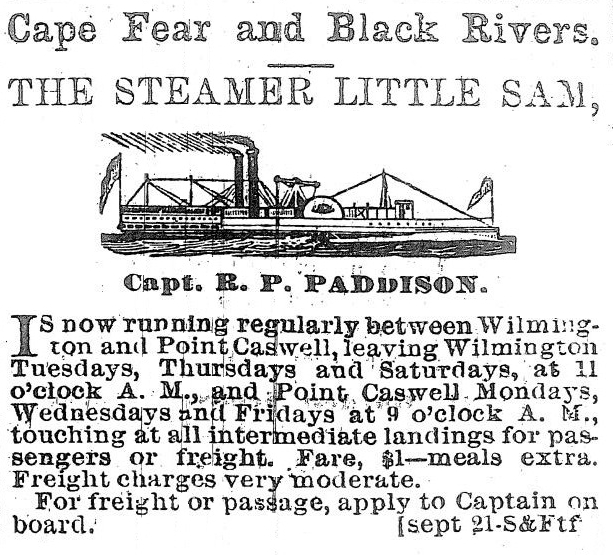
\includegraphics[scale=.9]{steamer_little_sam_ad_carolina_farmer_and_weekly_star_6_january_1871}\newline
  \textsc{---Carolina Farmer \& Weekly Star, 6 January 1871}
\end{figure}

The \steamer{Little Sam} must not have been too profitable.  An
economic recession slowed trade into 1873, but more important, Point
Caswell, named for Governor Richard Caswell (1729-1789), had not % chktex 8
developed as a steamboat center.  For many years before the Civil War
it had been a pole boat stop and a receiving point for farm and forest
products of the surrounding community.  In 1860, an advertisement in
the Wilmington \textit{Journal}, offering lots for sale, described it
as a ``thriving village'' on the Black River to which ``about 20,000
barrels are hauled annually.''  Yet it had no turpentine distillery.
\citep[4-2-1860]{wj}.\par

Post-war development of the town led to its incorporation in 1883, but
its charter was repealed in 1901.  \citep[389]{powellws}.\par

Paddison\index{Paddison, Captain R.~P.} was looking for a more
profitable situation.  So, perhaps by his encouragement, in 1874 the
\steamerco{Tar River Navigation Company} built the steamer
\steamer{North East}, and early the following year, with Captain
Paddison as her master, she was running a three times a week schedule
on the Tar River between Tarboro and Washington.  He begged farmers of
several counties served by the river for their patronage to keep
``freights on home produce at the very lowest rates.''
\citep[1-8-1875]{ts}.  But, within eight months, Paddison had returned
to the Black River, bringing with him the steamer \steamer{North East}.
\citep[9-24-1875]{ws}.  By this time, Point Caswell had obtained a
turpentine distillery and a sawmill and was fast becoming Pender
county's largest town.\par

The general economy had improved and the business at Point Caswell
increased to a point that the \steamer{North East} was kept busy.
Paddison\index{Paddison, Captain R.~P.} ran some excursions, but others
he had to turn down.  Upon one occasion, one suspects to promote
business, he took a ``select party of ladies and gentlemen'' from
Point Caswell to Maultsby's Point, ``a favorite resort of the young
people of that vicinity.''  The fare consisted of dancing in the
morning, ``a splendid repast,'' and dancing on board the boat all the % chktex 38
way home.  The party left the boat ``to complete the dance at
Dr.\ Hawes' that night.''  \citep[8-8-1876; 6-30-1876]{ws}.\par

Meanwhile, there was ``considerable activity among the farmers and
naval stores getters in the lower parts of Duplin, Sampson, and
Bladen'' counties.  \citep[2-18-1876]{ws}.  The \textit{Wilmington Star}
announced that a second steamer had been introduced to the Black River,
this one to the upper part, high up among the snags, sunken logs, and
flats in Sampson County.  Her owner and master was ``Commodore''
Charles Howe\index{Howe, ``Commodore'' Charles} of Franklin Township,
which had been part of New Hanover County before formation of Pender
in 1875.  The steamer, called \steamer{Little Adrian} in honor of
Aldrich Adrian of the Wilmington business firm of Adrian \& Vollers,
was 85 feet long and 35 feet wide.  \citep[11-19-1875]{ws}.  Flat
shaped, she must have been of shallow draft to navigate the shallows
of the upper river.\par

\section{The Black River Monopoly}

Shortly afterwards, the \steamerco{Black River Navigation Company},
with Howe\index{Howe, ``Commodore'' Charles} as one of the principal
incorporators, was formed.\footnote{Besides Howe, the incorporators
  were Alfred Martin\index{Martin, Alfred}, John C.
  Meyer\index{Meyer, John C.}, Haywood Boykin\index{Boykin, Haywood},
  E.~S.~Ward\index{Ward, E.~S.}, John Smith\index{Smith, John}, and
  Henry Vollers\index{Vollers, Henry}.}  The 1876-77 state legislature % chktex 8
granted the company the exclusive right to navigate steamers on the
Black River above Point Caswell for fifty years.\par

The act provided that ``in order to induce and enable the said company
to clear and improve and render fit for steamboat navigation on the
waters of the Big Coharie and Black River above the point on the
Black River at which such navigation is now practicable, the company
shall have the sole and exclusive right and privilege to navigate the
rivers with steamers from Point Caswell to all points up the Black
River and the Big Coharie for the period of fifty years \ldots The act
further provides that unless the company shall complete the
improvements mentioned as far up as Lisbon, to a degree sufficient to
render steamboat navigation safe and beneficial to the public within
five years from date the company shall forfeit all its rights,
privileges, and franchises.''  \citep[2-12-1886]{ws}.\par

The company seems to have done little or nothing to improve the river
and to capture the upriver trade.  It faced two major obstacles.
Harvesting of naval stores in the area had not reached large
proportions attendant with activity of turpentine barons, and the
small and independent farmers may have been reluctant to shift from
rafts and pole boats which cost them little more than their time.
But, more importantly, the magnitude of such an undertaking was not
generally realized until the Corps of Engineers commenced their
improvements a decade afterwards.  Thus, the company's monopoly was
allowed to expire by default without any attempt to renew it.\par

Instead, the company turned its attention to the navigable lower
river, putting its money into the acquisition of the steamer
\steamer{Isis}.  With Captain
S.~W.~Skinner\index{Skinner, Captain S.~W.} as her master, she made
regular runs between Point Caswell and Wilmington.  \citep[1-10-1879]{ws}.\par

Fire had destroyed Captain Paddison's\index{Paddison, Captain R.~P.}
five-year-old \steamer{North East}, causing ``considerable
inconvenience to shippers, who are compelled to resort to the use of
flats to move their produce.''  \citep[1-10-1879]{ws}.  Inasmuch as no
further mention is made of the \steamer{Little Adrian} one is left to
wonder if she had not fallen victim to a snag of the upper river.\par

\section{Steamer Service Returns to the Northeast River}

Meanwhile, efforts to restore steamboat service on the Northeast River
were thwarted by obstacles.  In April 1879, the Wilmington
\textit{Star} reported, ``The steamer \steamer{Clinton} arrived here
(Wilmington) yesterday from Bannerman's Bridge, with a cargo of 700
barrels of rosin.  A few months ago, the \steamer{Clinton} was a mere
wreck, but thrift and go-aheadativeness led by Bisby\index{Bisby} to
suppose that he could make her pay.  He is doing it, and it is the
kind of energy which we need right here and now.  Hundred of
unemployed and complaining might improve their conditions and secure
at least a competency by determined efforts like this energetic and
deserving mechanic.''  \citep[4-4-1879]{ws}.  Six months later, the
\steamer{Clinton} replaced the \steamer{Isis} on the Point Caswell and
Wilmington run, releasing the \steamer{Isis} to the Cape Fear to
substitute for the \steamer{Wave} which was being overhauled.
\citep[10-31-1879]{ws}.\par

\section{A Projected Steamboat-Railroad Line}

While the \steamerco{Black River Navigation Company} was obtaining its
monopolistic charter to operate above Point Caswell, a group of Point
Caswell business men, led by Captain R.~P.\
Paddison\index{Paddison, Captain R.~P.}, was promoting an alternate
scheme to bypass the river obstructions in tapping the upriver
commerce.  In April 1877, the \textit{Magnolia Record} reported that
the plan was to build a narrow gauge railroad from Point Caswell to
Clinton, touching at important points along the way, thus opening up
commerce several miles above Lisbon and deep into the pole boat
country.\par

The \textit{Record} reported that the country through which the road
would pass was ``very isolated'' and the ``crooked shallow streams''
were ``totally inadequate to assist the people in marketing their
produce.''  The project was justified by the ``inexhaustible
quantities of ton timber, forrests of crude turpentine, tar, shingles
\ldots which the inconvenience to market have kept almost intact, to
say nothing of the immense products of the farms.''
\citep[4-20-1877]{ws}.  At Point Caswell, steamships would be made
available to transport freight to Wilmington.\par

However, railroad plans were put on the shelf for four years while
Captain Paddison\index{Paddison, Captain R.~P.} occupied himself with
the steamboat business.  He lost the old \steamer{North East} to fire
in 1879; but early in 1880 he had built and was running a new and
larger steamer, the \steamer{John Dawson}, \citep[4-20-1880]{ws}, the
second boat bearing that name to run the Cape Fear and her
tributaries.  At first, the \steamer{Dawson} made regular runs between
Point Caswell and Wilmington, but soon she was competing for the Cape
Fear freight business.\par

It was in 1882 that Captain D.~J.~Black\index{Black, Captain D.~Jasper},
at age of sixteen, began work on the \steamer{John Dawson}.
\citep{shumpertsb}.  Black, a pioneer on the upper Black River, would
stick with river boats for forty-five years before retiring in
1928.\par

\section{New Move for Steamboat-Railroad Line}

In 1881, with the upper Black River as isolated as ever, the movement
to construct the Point Caswell to Clinton Railroad by way of Black
River Chapel and Lisbon\footnote{Black River Chapel was near present
  Ivanhoe and Lisbon near the confluence of the Great Coharie and Six
  Runs.} was resumed with vigor.  Leading business men of Sampson and
Pender counties formed committees to solicit \$50,000 in stock to
construct a forty-five mile long narrow gauge railroad and to acquire
a line of steamers to be based at Point Caswell.  In October 1881, the
Wilmington \textit{Star} reported that ``from present appearances it
certainly looks as if the \textit{iron horse} was destined to go
snorting through the huckleberry bushes and awakening echoes of the
Coharies before many more moons have waxed and waned.''
\citep[10-14-1881]{ws}.\par

For several months, meetings were held at Clinton and several points
along the proposed route rallying financial support of business men.
Then in February 1883 the state legislature chartered the road and
authorized the sale of \$150,000 capital stock.  The charter required
that the road be completed within two years.
\citep[51]{reillyjs}.\par

The following June, Paddison\index{Paddison, Captain R.~P.} was
awarded the contract to build the road.  \citep[6-1-1883]{ws}.\par

But when construction of the railroad seemed a near certainty,
Wilmington and Weldon Railroad\index{Wilmington and Weldon Railroad}
interests quietly contacted key Clinton business men and let it be
known that that company would consider building a branch line from its
main line at Warsaw to Clinton.  This served to divide the supporters
of the Point Caswell project.  This division grew even wider when some
of the promoters proposed ``a railroad to Raleigh, as nearly as
air-line as possible.''  \citep[10-26-1883]{ws}.\par

Paddison\index{Paddison, Captain R.~P.} and his loyal supporters
sought to crush this division with action.  About ten miles of
right-of-way was cut on each end of the proposed line.
\citep[10-10-18813]{ws}.  However, Clinton's support of the Point
Caswell line diminished while support for the Warsaw connection
increased.  Clinton's support and patronage was deemed necessary, and
support at other points dried up.\par

The Wilmington and Weldon Railroad\index{Wilmington and Weldon Railroad}
completed its spur line in 1886, and in April 1887 Clinton held a
joyous celebration attended by four to five thousand people.
\citep[4-20-1887]{ws}.\par

\chapter{Small Steamboat Prospers}

\textsc{Meanwhile}, the \steamerco{Black River Navigation Company} permitted
the upper Black River to continue in its wild state.  Nonetheless,
independent steamboat men found ways and means to provide service.  By
1886 the stream had four steamers, the same number as were serving the
Cape Fear River between Wilmington and Fayetteville.  In August 1886
the Wilmington \textit{Star} listed these as the \steamer{Delta},
Captain Hubbard\index{Hubbard, Captain} as master; the
\steamer{Lisbon}, Captain Black\index{Black, Captain D.~Jasper}; the
\steamer{Excelsior}, Captain Burkhimer\index{Burkhimer, Captain}; and
the \steamer{Susie}, Captain Snell\index{Snell, Captain}.  In
addition, there were five flat boats transporting naval stores and
other commodities.  They were Sessoms' and Lon (Lunch) Johnson's of
Beatty's Bridge, Bladen County; Johnson \& Sons' and Herring \&
Peterson's of Ingold on the Great Coharie, Sampson County.
\citep[8-13-1886]{ws}.\par

The following year, Captain Bixby\index{Bixby, Captain W.~H.} of the
U.~S.\ Corps of Engineers explained that the Black River served a
large area.  With its tributaries it had ``a total length of about 175
miles and drainage area of about 1,547 miles.''  He noted that it was
obstructed by seven bridges ``allowing about 14 feet clearance above
low mean water,'' but these''will probably be provided with draws at % chktex 38
expense of local authorities.''  \citep[8-12-1887]{ws}.\par

\section{A.~J.~Johnson, Promoter}

By now, steamboats and steam-flats were being built to specifications
for the upper Black River trade.  A.~J.\ Johnson\index{Johnson, A.~J.},
a native of the Taylor's Bridge community on Six Runs in Sampson
County, was one of the chief promoters of steamboat transportation.
He began about 1880 and continued for thirty-four years until his
death in 1914.\par

Johnson\index{Johnson, A.~J.} was a business man who became involved
in the turpentine industry and thus had a personal need for regular
and dependable steamboat service.  Although he was not a steamboat
captain himself, he saw that good boats were put in the hands of good
masters.  Foremost among these was D.~J.\ Black\index{Black, Captain D.~Jasper}
of Point Caswell who was captain of the stern-wheel steamer
\steamer{Lisbon} when he was twenty years old.\par

The story of the \steamer{Lisbon} became one closely associated with
the advancement of steam navigation in the wild Black River country;
and some of Captain Black's adventures with her are as intriguing as
storybook fables.\par

The way that Captain D.~J.\ Black\index{Black, Captain D.~Jasper} and his
black playmate Henry Cromartie\index{Cromartie, Henry} took to
steamboating is one of these stories.\par

Black's parents moved to Point Caswell, and when he was fourteen he
and Cromartie were doing chores for the residents of the village.  At
times they worked for Captain R.~P.\ Paddison\index{Paddison, Captain R.~P.}.
One day, the Captain arrived with the steamer \steamer{John Dawson}
loaded with freight and no one to unload her.\par

``Would you boys like a man size job with a man's pay?'' he asked
young Jasper and Henry.\par

They were ready.  After the freight had been unloaded he asked,
``Would you boys like to work on the boat?''\par

``Yessir!'' they eagerly chimed.  They proved trustworthy as well as
eager, and soon they were running the boat for Captain
\textit{Dick}.\par

As they moved up together, Black\index{Black, Captain D.~Jasper}
became captain and eventually owner and Cromartie\index{Cromartie, Henry}
stood at his side as pilot.\par

They remained inseparable during their long careers on the river.
\citep{blackj}.\par

Luther Sherman\index{Sherman, Captain Luther}, an accomplished ship's
carpenter, built the \steamer{Lisbon} at Point Caswell in 1880.  He
was to build many other steamboats at that place.  When she was
``thoroughly overhauled'' in 1884 was the property of
A.~J.\ Johnson\index{Johnson, A.~J.}.  \citep[7-4-1884]{ws}.  She had
been making regular runs between Lisbon, a Sampson County business
center on the Great Coharie, and Wilmington.\par

But, during the overhaul, Johnson had twenty feet added to her length
and put her on a run between Clear Run, twelve miles below Lisbon,
where he had built a turpentine distillery, and Wilmington.
\citep[7-14-1884]{ws}.  But the town of Lisbon did not immediately
lose her steamer lifeline.  Captain R.~P.\
Paddison\index{Paddison, Captain R.~P.} put his screw propelled 45 ton
steamboat \steamer{Excelsior} on the Black River run to Lisbon.
\citep[2-27-1885]{ws}.\par

\section{Black River Improvements}

The ``indomitable'' Captain Paddison\index{Paddison, Captain R.~P.}
was politically active, and he used his influence to obtain
improvements for the Black River country.  In August 1883 he took
Congressman Green on a special steamboat trip up the Black River to
the head of navigation.  Traveling at two miles an hour, he pointed
out the hazards and difficulties that steamboat men faced in
navigating the stream.  \citep[8-24-1883]{ws}.  Two months later Green
had in his hands a memorial to Congress from the people of Bladen,
Pender, and Sampson counties asking for an appropriation to improve
the river.  It explained: ``There is at present about seven hundred
and fifty thousand dollars in produce annually transported to market
on these waters, consisting of cotton, naval stores, lumber, shingles,
etc., and we confidently feel that if the rivers are put in navigable
condition this amount would be doubled.''  \citep[11-2-1883]{ws}.\par

In January 1885 the \steamer{H.~B.~Wright}, a new government steamer
built at Fayetteville and put under command of Captain Flowers, went
on a surveying expedition of the Black River.  Out of this came a
report by Captain Bixby\index{Bixby, Captain W.~H.} of the U.~S.\ Corps
of Engineers recommending extensive improvements to provide ``a
thoroughly cleared channel of natural depths over the seventy miles
\ldots from its mouth to near Lisbon'' was recommended by Bixby the
following year.  \citep[2-16-1886; 8-12-1887]{ws}.\par

\section{Howes Seek to Invoke Monopoly}

Once it was evident that the U.~S.\ Corps of Engineers would make
major improvements to the Black River and thus make it more suitable
for steamboat use, two Pender County brothers, Charles\index{Howe, Charles}
and William Howe\index{Howe, William}, sought to invoke the fifty-year
monopoly which the 1876-77 state legislature had granted to the % chktex 8
\steamerco{Black River Navigation Company}, claiming that they held
the company's charter.  They began demanding tolls of steamboats
passing upstream by their landing at Howe's Bluff.\footnote{Howe's
  Bluff may have been the same as present Haw Bluff near the mouth of
  Mill Creek and a short distance below the river's `Narrows.'}
Inasmuch as the necessary improvements had not been made as required
by the legislative act, the monopoly had been void after five years.
So, steamboat men declined to pay tolls, whereupon the Howes built a
boom across the river at Howe's Bluff to prevent passage of their
steamboats.\par

When the steamer \steamer{Delta} was denied passage, her owner,
Captain J.~D.\ Kerr\index{Kerr, Captain J.~D.} of Sampson County,
brought indictments against the Howe brothers, charging them with
preventing free navigation of the river, a public stream.  Two Pender
County justices of the peace, George D.\ Larkins and E.~A.\ Hawes,
found the defendants guilty as charged and ordered that they spend
twenty days each in jail at Wilmington.  Their attorney gave notice of
appeal to the Pender County Superior Court, \citep[2-12-1886]{ws}, but
they're is no record of the case reaching that court.  That the
monopoly was generally regarded as invalid is indicated by the
increased activity of steamboats on the upper Black
River.\footnote{The monopoly's excessive length seems to have smacked
  of opportunism as often found after the Civil War.}\par

\section{Prosperity on the Black River}

Although Wilmington's naval stores receipts had begun to show a
substantial decline by 1888 \citep[2-4-1889]{ws}, cleaning out of the
Black River by the U.~S.\ Corps of Engineers brought increased
activity and prosperity to the once isolated Black River country.\par

Opening of the Wilmington to Fayetteville link in the Cape Fear and
Yadkin Valley Railroad\index{Cape Fear and Yadkin Valley Railroad} in
1890, paralleling the Black and South rivers, seems to have reduced
very little the flow of naval stores by water.  If there was any loss,
this was more than compensated by increased shipping of other
commodities by increasingly prosperous farmers.  Despite the panic of
1893, the last decade of the 1800's saw an unprecedented surge of
business activity on the Black River.\par

A year after the 1893 panic, a brief item in the Wilmington
\textit{Weekly Star} revealed that steamboat men were not suffering
from an old problem of too little up-freight: ``The steamboat
\steamer{Lisbon}, Capt. Black\index{Black, Captain D.~Jasper} of the
Black River line, had more up-freight than he could carry.  The boat
was loaded down to the guards with groceries and other merchandise for
Clear Run and other points on the river, and left lots of freight on
the wharf.  This shows that times are not so hard in the huckleberry
country as in other sections.''  \citep[5-18-1894]{wws}.\par

\section{Steamboat Numbers Increase}

The 1880's brought a large increase in the number of steamboats built
for the upper Black River.  In 1882 a little steamer, the 25 to 30 ton
stern-wheel \steamer{Lisbon (I)}, which ran most of her fifteen years
under Captain D.~J.\ Black\index{Black, Captain D.~Jasper}, was
constructed.  Upon retirement she was succeeded by a new and larger
steamer with the same name.  She proved to be profitable, and Captain
Black built a second small boat, the \steamer{Hall}.
\citep[2-26-1970]{sa}.  He, however, sold her after running her on the
Black River for a short time.  Then he built the \steamer{Magruder},
which he also sold.\par

\steamer{Lisbon (II)}, like \steamer{Lisbon (I)}, was a stern-wheel
steamer.  She was built by Captain Black near Point Caswell and put in
service in November 1887.  She was 88 feet long, 19 wide, and four
deep and was capable of carrying 350 barrels of naval stores.  Thus,
she was of about 50 tons.  \citep[11-5-1887]{ws}.\par

In 1885 Captain J.~D.\ Kerr\index{Kerr, Captain J.~D.}, a Sampson
County merchant, built the small stern-wheel \steamer{Delta} and named
her for a river landing and small community near present Ivanhoe where
he operated a general store.  \citep[4-29-1887]{ws}.  With Captain
Hubbard\index{Hubbard, Captain} as her master, she was running both
the Black and Northeast rivers.  \citep[4-30-1886]{ws}.  In April 1887
she exploded her boiler killing two men.  Captain Kerr sold the wreck
to Captain Herbert Ward\index{Ward, Captain Herbert}, who repaired her
and returned her to service running on several Cape Fear tributaries,
including the Black River and Town Creek.  \citep[2-22-1889; 8-15-1890]{ws}.\par

The \steamer{Excelsior}, a small experimental steamer, appeared on the
Black River in 1884.  Built by Captain H.~P.\
Bowdoin\index{Bowdoin, Captain H.~P.}, she was designed to navigate
during low water beyond the range of the ordinary steamer.  Her
builder gave her a screw propeller ``adjustable to any depth of water
not less than thirteen inches.''  Steamboat men up and down the Cape
Fear and her tributaries were very interested in the ``peculiar
character of her construction.''  \citep[4-25-1885]{ws}.\par

Soon after \steamer{Excelsior}'s trial run, Captain
Bowdoin\index{Bowdoin, Captain H.~P.} headed up the Black River and
made it to Lisbon on the Great Coharie, a point which had been reached
by Captain Paddison\index{Paddison, Captain R.~P.} with his steam
flat.  \citep[2-27-1885]{ws}.\par

The steamer ran the Black and Cape Fear rivers only a short time.  In
April 1885, she burned on a run between Wilmington and Fayetteville
with the builder's son, Captain H.~L.\ Bowdoin\index{Bowdoin, Captain H.~L.},
as her master.  \citep[4-17-1885]{ws}.  However, she seems to have
been rebuilt and returned to service.  Captain
Burkhimer\index{Burkhimer, Captain} was running her on the Black River
in 1886.  \citep[10-13-1886]{ws}.\par

Late in 1886, Captain H.~P.\ Bowdoin\index{Bowdoin, Captain H.~P.},
``turned out a new craft in the shape of a steam-flat'' to be run
between Wilmington and Long and Town creeks.  He named her the
\steamer{Enterprise}.  \citep[4-29-1886]{ws}.  A year later, she was
running the upper Black River with Captain C.~P.\
Moore\index{Moore, Captain C.~P.} as her master,
\citep[2-29-1887]{ws}, and in 1889 she and the \steamer{Delta} were
running as a line between the Delta and Wilmington.
\citep[2-22-1889]{ws}.\par

In August 1890, the ``new Black River steamboat \steamer{Maggie},'' % chktex 38
with Captain William Skinner\index{Skinner, Captain William} as
master, made her trial run from Wilmington to Clear Run, Sampson
County.  ``She had no freight nor passengers, but had two flats in
tow.''  Yet her owners, \steamerco{George Harris Son \& Company}
contemplated running her regularly.  \citep[8-1-1890]{ws}.  But, by
now, steamboat service had become well established along all the
navigable areas of the river, and the new steamer must not have
attracted enough business to show a profit.  Eighteen months later,
she was sold at auction for \$1,100 to L.~S.\ Ehrich of Georgetown,
South Carolina.  \citep[1-29-1892]{ws}.\par

\begin{figure}[h]
\centering
  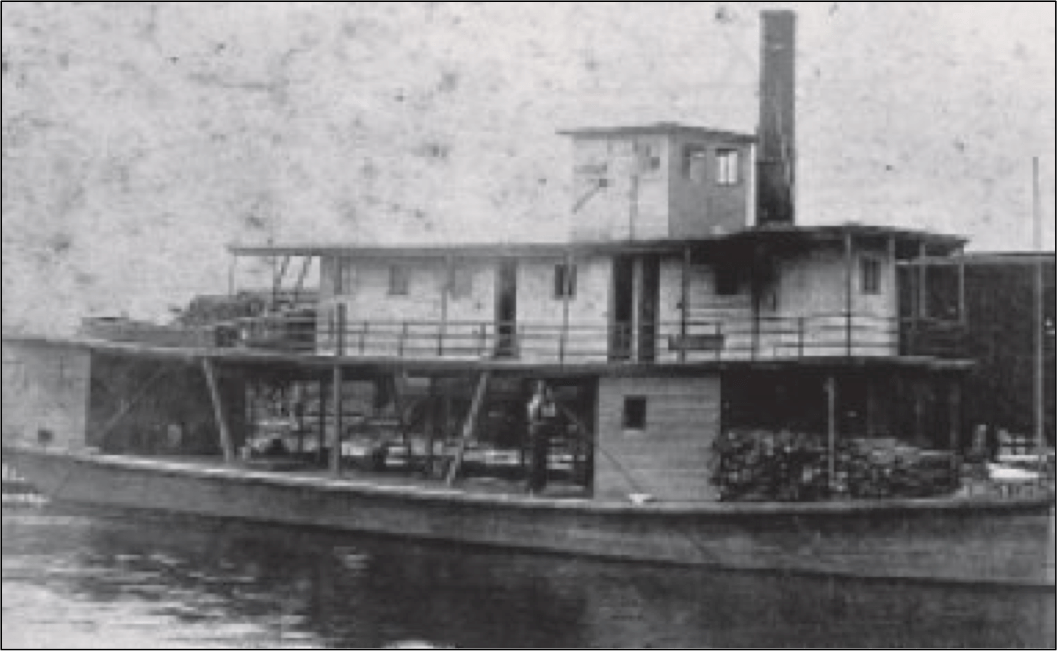
\includegraphics[scale=.5]{steamerlisbon}\newline
  \textsc{The Lisbon}---D.~Jasper Black
\end{figure}

\begin{figure}[h]
\centering
  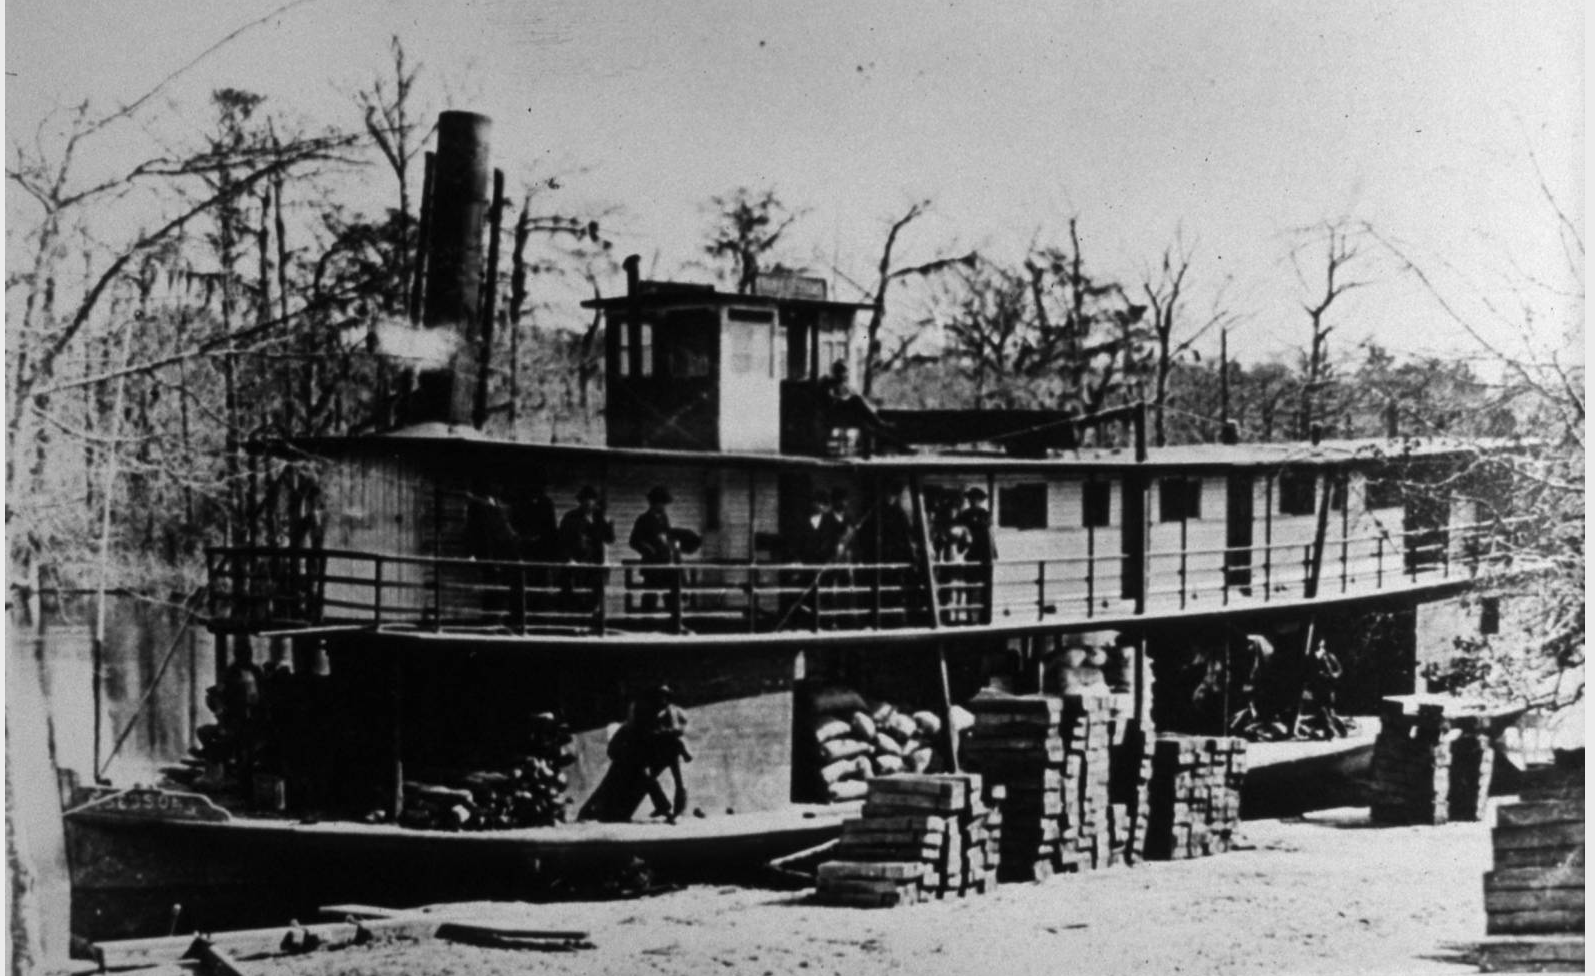
\includegraphics[scale=.2]{frank_sessoms_0}\newline
  \textsc{The Frank Sessoms}---D.~Jasper Black
\end{figure}

\section{The Frank Sessoms}

The \steamer{Frank Sessoms} was built by Luther
Sherman\index{Sherman, Captain Luther} of Point Caswell in 1894
``under the personal supervision of her owner and master,
Capt. D.~J.\ Black\index{Black, Captain D.~Jasper}.''  Although she
was built for the Black River, she was of 75 tons and was about twice
the size of \steamer{Lisbon (I)} and other small steamers navigating
these waters.\par

The \textit{Wilmington Star} stated that she was ``brand new from stem
to stern \ldots{} 100 feet long, 22 feet wide, draught 16 inches,'' % chktex 38
and she had a freight capacity of 500 barrels.  She had ``ample
accomodations for passengers, saloons, and berths on the upper deck
nicely furnished.''  \citep[1-16-1894]{ws}.  Two old steamboat men,
Captains Sherman\index{Sherman, Captain Luther} and
Driver\index{Driver, Captain William}, were quoted as saying she was
the ``best boat of her class ever on the river.''
\citep[1-23-1894]{ws}.  She was given the name of a merchant who
operated a general store at Long View on the Black River.\par

The \steamer{Frank Sessoms} made her first trip up the Black River to
Mill Creek where Ed Hawes and Ed Sellers had opened a general store,
built a turpentine distillery, and were serving Bladen and Pender
County patrons.  But, she was too large to proceed further upstream;
and her patronage was limited to the lower river and the Cape Fear.
\citep[1-23-1894]{ws}.  Three months later, she was making regular
runs between Wilmington and Fayetteville for the
\steamerco{Cape Fear Transportation Company} and with Captain Irving
Robeson\index{Robeson, Captain Irving} as her master, taking the place
of the wrecked \steamer{Cape Fear}.  By 1896, Captain Herbert
Ward\index{Ward, Captain Herbert} was her master, and he served until
1899 when the Cape Fear company sold her to Mark Moses of Georgetown,
South Carolina for \$3,000.  She was put on the Santee River as a
freight boat.  \citep[7-14-1899]{ws}.\par

\section{The E.~A.~Hawes}

The \steamerco{Cape Fear and People's Steamboat Company} maintained a
strong bid for Black River freight throughout the 1890's.  In 1895,
the steamer \steamer{E.~A.~Hawes}, named for a Black River business
man, was constructed by Captain Ellis Sherman\index{Sherman, Captain Ellis}
at Point Caswell ``for Black River.''  \citep[11-22-1895]{ws}.\par

Slightly larger than the smaller steamers, she was 80 feet long and 18
feet in beam.  \citep[9-27-1895]{ws}.  She was to have several masters
who had seen service with the Cape Fear line.  Soon after her
launching, Captains Herbert Ward\index{Ward, Captain Herbert} and
D.~J.\ Black\index{Black, Captain D.~Jasper} were taking her on
regular runs to Clear Run.  And, in 1899, when Captain Black resigned
from the Cape Fear company, after seventeen years continuous service,
he was replaced by Captain James C.~Smith\index{Smith, Captain James C.}
of Wilmington and Fayetteville who had been master of the steamer
\steamer{Compton}.  \citep[7-7-1899]{ws}.\par

The \textit{Hawes} made frequent freight runs on the Cape Fear River
and some of her tributaries until she sank at the wharf in Wilmington
in January 1901, having arrived a few hours earlier with a heavy
freight, including 330 barrels of rosin from Hallsville on the
Northeast River in Duplin County.  She was raised and towed to
Fayetteville for repairs and returned to service.
\citep[1-11-1901]{ws}.  In 1905 with Captain
Robeson\index{Robeson, Captain Irving} as master, she was running
between Wilmington and Fayetteville.  \citep[marine intelligence]{ws}.\par

\section{The A.~J.~Johnson}

The \steamer{A.~J.\ Johnson} was one of the more successful steamboats
to run the Black River.  In 1899 ``a number of Black River substantial
business men'' in the form of trade assurances backed the construction
of a 57-ton stern-wheel steamer to serve Sampson County together with
points along the lower river.  \citep[12-9-1888]{ws}.\par

Named the \steamer{A.~J.\ Johnson} for a Sampson County business man,
the boat was built at Clear Run by John B. Robinson\index{Robinson, John B.}
under Johnson's direction and towed to Wilmington where she received
new and improved machinery at Skinner's ship yard.
\citep[12-22-1899]{ws}.  An item in the December 22 Wilmington
\textit{Star} stated that she was owned jointly by Robinson and James
W.~Marley\index{Marley, James W.} of Clear Run.
\citep[12-22-1899]{ws}.  Soon afterwards, Johnson had acquired their
interests.\par

A 1909 inspection certificate issued by the Steamboat Inspection
Service of the Department of Commerce and Labor out of the Port of
Charleston, S.~C., states that the boat was owned by A.~J.\ Johnson,
and W.~H.\ Ward\index{Ward, Captain W.~H.} was her master.  She was
licensed to carry a crew of two pilots, two engineers, two firemen,
one watchman, four deck crewmen, and one steward.  She could carry
fourteen passengers, seven in second-class cabins and seven deck or
steerage.  A penned notation permitted the boat to navigate ``not
exceeding thirteen hours with one pilot, one engineer, one fireman,
four deck crew, one watchman, and one cook.''\par

In January 1900, the \steamer{A.~J.\ Johnson} made her trial run
between Wilmington and Clear Run with Captain
J.~S.\ Watson\index{Watson, Captain J.~S.} of Point Caswell as her
master.  A short while afterwards she was under the command of Captain
D.~J.\ Black\index{Black, Captain D.~Jasper}, also of Point Caswell.
Marine intelligence of 1905 lists Black as her master.\par

The \steamer{A.~J.\ Johnson} ran the Black River until the death of
A.~J.\ Johnson\index{Johnson, A.~J.} in 1914.  She was tied up at
Clear Run and sank soon afterwards during a violent storm.
\citep[2-26-1970]{sa}.  But a few years later, her boiler was salvaged
by John F.\ Johnson of Bladen County's Rowan community and installed
in his new steamboat \steamer{Brook}.  Her engine was salvaged by
Henry Hunt of Long View, Bladen County, and installed in his steamer
\steamer{Oast}.  \citep{johnsonwc}\citep{johnsonlg}.\par

\chapter{Decline and the End}

\textsc{Forebodings} of a decline in steamboat business became a
reality soon after 1900 and slowly brought to an end the steamboat era
in lower North Carolina.\par

The last ``inexhaustible'' source of naval stores upon the once remote
Black River slowed to a trickle as the turpentine barons dripped the
great pine forests dry.  Small villages grew up around the stations of
the Cape Fear and Yadkin Valley Railroad between Wilmington and
Fayetteville, and new businesses located at these points while
business upon the river withered.  Somewhat belatedly, in 1911, the
railroad came to Elizabethtown, onetime an important steamboat station
on the Cape Fear River.\par

Steamboat men, wedded to the river, put up a determined fight until
losses to the railroads were compounded by losses to the motor truck.
They cut operating costs and for a time found new business in a
changing and growing economy.  Veteran Captain
D.~J.\ Black\index{Black, Captain D.~Jasper} remained on the Black
River until 1926; and Captain Henry Hunt\index{Hunt, Captain Henry}
rendered passenger and freight service on the Cape Fear River until
about 1939.\par

\section{The Charles M. Whitlock}

The \steamer{Charles M. Whitlock}, an 85-foot-long screw propelled
steamer built in 1901 by Captain Ellis Sherman\index{Sherman, Captain Ellis}
of Point Caswell, was one of the first twentieth century Black River
boats, and she was the last, retiring with Captain
D.~J.\ Black\index{Black, Captain D.~Jasper} in 1926.
\citep[7-5-1901]{ws} \citep{shumpertsb}.\par

She was named for a popular Missionary Baptist preacher of Wilmington;
and upon retirement she was tied up at Hammie Marine
Railway\index{Hammie Marine Railway}.  Her engine was junked, her
upper structure fired the railway's boiler, and the Corps of Engineers
sank her hull.  \citep{blackj}\citep{wardmb}.\par

She began service as a passenger and freight boat on the Black River
and Town Creek.  In 1905, Captain Sherman\index{Sherman, Captain Ellis}
sold her to T.~J.\ Gore\index{Gore, T.~J.} at which time she was
reconditioned and cabins provided for both white and colored
passengers.  A new paint job made her ``as pretty as a butterfly in
May.''  She was put on runs between Wilmington and Point Caswell and
Wilmington and Lillington\footnote{The village of Lillington is now Long Creek}
on the Long Creek with M.~B.\ Ward, Sr.,\index{Ward, Captain M.~B.\ Sr.} as
master and W.~H.\ Ward\index{Ward, W.~H.} agent.  \citep[10-6-2905]{ws}.\par

Some time afterwards she was purchased by J.~W.\ Brooks, a Wilmington
wholesale merchant, to deliver merchandise to his patrons and to
render passenger and general freight service; and years afterwards she
was purchased by Captain D.~J.\ Black\index{Black, Captain D.~Jasper}.
At various times, Captains W.~P.\ Blizzard\index{Blizzard, Captain W.~P.}
and John Lewis\index{Lewis, Captain John} served as her master.\par

\section{The Alice}

In 1903, a boat similar to the \textit{Whitlock} was built by Captain
Luther Sherman\index{Sherman, Captain Luther} at Tar Landing on
Moore's Creek for Peter Simpson\index{Simpson, Peter}, ``a hard
working, energetic Negro,'' who was engaged in lighter and wood % chktex 38
business.  The screw propelled steamer was named for Pete's wife.
\citep[11-6-1903]{ws} \citep{wardmb}.\par

Simpson engaged Captain John Lewis\index{Lewis, Captain John} as
master and ran the \steamer{Alice} on the Black River and Long Creek
in competition with the \steamer{Charles M. Whitlock}.  After several
years, he sold her to Captain Snell\index{Snell, Captain} of Norfolk,
Virginia; and with Ed Tharp\index{Tharp, Ed} as engineer, Snell ran
the steamer on the Black River and Town Creek.  She was last run by
J.~W.\ Brooks, who retired her in 1919 when she failed inspection by
the Department of Commerce and Labor due to a rotting hull.
\citep{johnsonjf}\citep{cavalieril}\citep{wardmb}.\par

Born in 1856, a son of a Cape Fear River captain, unlettered Lunch
Johnson\index{Johnson, Lunch} was a man of the river who taught his
three sons---Willis, Jessie, and Henry---the steamboat business.  One
son, Willis\index{Johnson, Willis}, continued the family
tradition.\par

In 1886, at the age of thirty, Lunch Johnson had located on the Black
River and was doing business on his own with a steam flat.  By 1900,
he was operating the flat \steamer{Worth J.}, a one deck screw
propelled craft which he later sold to Roonie Skipper\index{Skipper, Roonie}
and replaced with a small screw propelled steamboat, the
\steamer{Buisy Bee}, which he and his sons built near their home at
Strawhorn Landing.  Meanwhile a steam flat, \steamer{Black River}, was
built for son Willis to run upon the upper river.\par

Although Johnson was ``a good business man'' as well as ``a good boat
man'' his last decade on the river was a time of struggle to make a
profit.  With naval stores freight a mere memory, he went after the
farm business, hauling virtually anything and everything that the
farmer wanted moved to and from market.  On her stern, the steamer had
stalls for cattle and pens for hogs; often, one might see crates of
chickens, ducks, and turkeys stacked in every available corner to the
second deck.\par

Meanwhile, Willis was piloting the steam flat \steamer{Black River}
far up into Sampson County, bringing down small lots of naval stores
together with increasing quantities of farm produce.  So they
continued until old age and poor health forced their retirement.  The
\steamer{Buisy Bee} was tied up at Strawhorn Landing and rotted at her
moorings.  \citep{johnsonwc}\citep{johnsonlg}\citep{wardmb}.\par

\section{The Gasoline Tug}
The gasoline tug appeared on the Black River soon after 1900 and
bright with it the advantage of economical operation.  Unlike the
steam tug and the steamboat, it did not require a licensed pilot.  Two
or three men could manage it and its tow.\par

However, it had a serious disadvantage; it did not have the pulling
power of the steam tug, and in some instances, it was used as a
supplement to steam craft, which were designed to take two or more
lighters in tow.\par

In 1902 Joe Beatty\index{Beatty, Joe}, a business man near Beatty's
Bridge, built his gasoline powered tug \gastug{Nellie Blythe}; but
soon afterwards, he replaced her with the steam flat \steamer{Pioneer}
which he used for freighting until 1915 when he sold her to Henry
Hunt\index{Hunt, Captain Henry} of Long View for freight service on
the Northeast River.  Hunt renamed the craft the
\textit{Oast}\index{Pioneer,~steamer}.\par

In 1917 three brothers---Campbell, Troy, and Lee Johnson of Bladen
County's Rowan community---built the gasoline tug \gastug{Montezuma}
at David's Landing, Black River, using the machinery from Bill
Corbett's\index{Corbett, Bill} \gastug{July}, for flat boat towage on
the Black and Cape Fear rivers for several lumber companies.  After
three years, the gasoline boat was replaced by a 35-ton steamer, the
\steamer{Brook}, also built at David's Landing for both freight
service and towage.\par

The \steamer{Brook}, with Campbell Johnson\index{Johnson, Captain Campbell}
as master and Lee Johnson\index{Johnson, Lee} as engineer, ran the
Black and Cape Fear rivers two years.  Naval stores freight had
disappeared, and most of the business was up-freight---fertilizer and
groceries and hardware---for a few merchants and farmers who were
still dependent on river transportation or found lower steamer rates
advantageous.\par

The \steamer{Brook} hit a snag and sank at the County Line on the Cape
Fear in 1922.  Inasmuch as she was not turning a good profit she was
sold to Alex Bordeaux\index{Bordeaux, Alex}, who converted her into a
steam tug and renamed her the \textit{Bostic}\index{Brook}.
\citep{johnsonwc}\citep{johnsonlg}.\par

\section{The Last Steamboat on the Cape Fear}

After World War I, steamboat business on the Cape Fear went into a
decline.  Singing of the \steamer{A.~P.~Hurt} brought an end to the
larger steamers.\par

But for nearly twenty years after the war, Captain Henry
Hunt\index{Hunt, Captain Henry} continued service with his stern-wheel
steamer \steamer{Thelma}, at first running between Wilmington and
Fayetteville and, later, Wilmington and Elizabethtown, making two
round trips a week.  The \steamer{Thelma} was idled about 1939 due to
the poor health of her owner and master.  For a good part of this time
the steamboat was a family enterprise, Hunt being assisted by his two
sons, Elmer and Tommy.\par

Today the \steamer{Thelma} is remembered with a degree of nostalgia by
many of the people who lived along the Cape Fear during the 1920's and
1930's.  Catering to passengers, she had ten staterooms on the second
of her three decks.  One of her Bladen County patrons recalls that the
fare from Kelly's Cove to Wilmington was seventy-five cents, and this
included supper and breakfast on the boat and lodging for the night.
\citep{pridgens}\citep{rawlsgw}\par

The \steamer{Thelma} was built in 1914 by Luther
Sherman\index{Sherman, Captain Luther} of Point Caswell for
J.~W.\ Brooks\index{Brooks, J.~W.}, the Wilmington wholesale merchant;
and Brooks sold her to Hunt\index{Hunt, Captain Henry} about 1922
after service was disrupted by the sinking of the \steamer{Brook}.\par

Before buying the \steamer{Thelma}, hunt had run the Black River for a
number of years.  He started with the \steamer{Annie B.}, a screw
propelled steamer 65 feet long, 14 feet wide, and five feet of hold,
which he named for his daughter Anna Belle.  In 1915, he purchased the
steam flat \steamer{Pioneer} from Joe Beatty\index{Beatty, Joe},
Changed her name to \textit{Oast}\index{Pioneer,~steamer} and put her
on the Northeast River as a freight boat.
\citep{johnsonwc}\citep{wardmb}.\par

In 1939, Hunt willed the \steamer{Thelma} to his son Elmer, and his
will was probated in 1941.  But Hunt's sons did not carry on the
business.  Both met accidental deaths, one before his own.  So, the
\steamer{Thelma}, the last of the Cape Fear stern-wheel steamboats,
fell victim to neglect and sank at her moorings near the bridge at
Elizabethtown.  \citep{rawlsgw}\citep{campbellws}\citep{bcw}
\citep[7-7-1973]{bj}.\par


\part{IV}

\chapter{Steamboat Disasters}

\textsc{Steamboat} travel on the Cape Fear and her tributaries was
safe.  Over a period of nearly a century, only about thirty-six lives
were lost in the eleven accidents which could be termed disasters.
The accidents included eight boiler explosions, two sinkings, and
firing of a Wilmington wharf resulting in the destruction of the
greater part of the business district.\par

The loss of life from lesser accidents was much greater and received
lesser notice.  Unfortunately many blacks, who comprised the larger
part of the crew of most steamers, could not swim, and often a man
overboard meant a man drowned.  And, it was not infrequent for a raft
or small flat boat to be caught in the wake of a passing steamer and
upset, causing loss of life.\par

Yet, a good part of the time, those traveling by steamer seemed to
harbor a dread of a boiler explosion.  There was but one explosion
with the loss of two lives during the first thirty-five years of steam
navigation on the Cape Fear; but, at times the newspapers were filled
with reports of disasters from other parts of the country.  Midway the
century the loss of life from boiler explosions and other accidents
was appalling.  During the first six months of 1852 the Wilmington
\textit{Journal} reported that no less than twenty steamers in the
United States had accidents in which 428 persons lost their lives and
many more were seriously injured.\par

Although it did not involve the Cape Fear or her tributaries, the
people of the Wilmington area in 1833 had an opportunity to view the
horrors which sometimes attended steamboat explosions it was the
explosion of the steamer \steamer{Pulaski} which in early June that
year was enroute from Charleston to Baltimore carrying a large number
of passengers.  She was to be at sea but one night, but that was to be
a horrible one.  When about 11 o'clock she burst her boiler off
Wilmington and sank.  The beaches about the mouth of the Cape Fear
were strewn with fragments of the wreck, and many bodies of the
drowned floated ashore.  Most were beyond recognition and were buried
on the sands in the sands of the shore.  \citep[3-14-1884]{ws}.\par

That the disasters made a deep impression on the public mind is
unquestionable.  Tales of horror became a part of the folk tradition
of the Cape Fear country and are retold to this day by some of the
older people.\par

Citing one example here, April 1887 the bridge tender at Point Caswell
on the Black River was roused from his slumber about two o'clock in
the morning.  A little steamer was running late and wanted to be on
her way.  The tender overheard the captain say, ``I'm going to be at
the Delta by daybreak or I'm going to blow her to hell!'' and a few
miles upriver she did blow.  She blew the fireman through the top of a
cypress tree leaving a tatter from his shirt danglig from a limb.
\citep{kellya}.\par

\section{The John Walker}

The first disaster on the Cape Fear River was in 1831.  The boat was
the \steamer{John Walker}, an early steamboat which had been named in
honor of one of Wilmington's more distinguished citizens.  She had been
put under command of Captain Alexander Dickson, who had piloted river
boats for many years.\par

The November 23, 1831, \textit{Cape Fear Recorder} reported that the
\steamer{John Walker} had but a few years of service and was regarded
to be in sound condition.  She was towing a vessel down the Cape Fear
River, and when but a short distance and in the vicinity of the Dram
Tree, a legendary maritime landmark, her boiler-engine exploded,
killing captain Dickson and Old Isaac, a well known black man who was
her engineer.  \citep[2-10-1882]{ws}.\par

\section{The Chatham}

It seems remarkable that the Cape Fear went from 1831 to 1853 without
a boiler explosion, that the pioneering steamers suffered no disaster.
Perhaps this was due to the lower horsepower of the machinery.  The
new generation of boats, however, were given more power and traveled
at higher speeds.\par

This good record was rudely interrupted in early August 1853 when the
\steamer{Chatham}, a stern-wheeler of the \steamerco{Cape Fear Line},
coming down from Fayetteville, blew one of her two boilers about
thirty miles below that city.  The black fireman was killed and two
other persons were injured, including the captain, who was blown
overboard with a broken arm.\par

The boat, loaded with naval stores, sank in seven foot water.
\citep[8-19-1853]{wj}\citep[8-17-1853]{rr}.  She was raised, returned
to service, and was running at the outbreak of the Civil War in
1861.\par

\section{The Tug Fayetteville}

The boiler of the steam tugboat Fayetteville\index{Fayetteville, steam~tug}
exploded in May the same year.  She sank inside the bar, but her engineer
and fireman, badly scalded, survived.\par

\section{Safety Devices}

A few months before the Cape Fear's steamboat safety record was marred
by the explosion of the boiler of the \steamer{Chatham} manufacturers
were advertising several safety devices in the Wilmington newspapers.
These included water and steam gauges and a fuseable metallic plug.
The plug was a simple and dependable device.  Made of lead and
inserted in the lower part of the boiler, it guarded against a quick
surge of steam pressure caused by water getting too low.  when
uncovered by water, the plug would melt and release the steam.
\citep[4-29-1853]{wj}.  If the plug melted when the boat was some
distance from her destination, the engineer could get her on her way
by cutting and skinning a green pine sapling and driving it into the
hole.  This makeshift plug would shrink when uncovered by the water
and pop out under rising steam pressure.  An engineer running on the
Black River in the early 1900's reports that he had two safety plugs
to melt on him due to the malfunction of a water pump.
\citep{johnsonlg}.\par




\begin{thebibliography}{99}

\section*{Books, Pamphlets, Theses, Papers}

\bibitem[\protect\citeauthoryear{Brickel,~J.}{1968}]{brickellj}
  Brickell, John.  \emph{The Natural History of North Carolina}, 1968
  reprint of 1737, Johnson Publishing Co., Murfreesboro, N.~C.

\bibitem[\protect\citeauthoryear{Clark,~W.}{1861-1865}]{clarkw}
  Clark, Walter.  \emph{North Carolina Regiments, 1861-1865}, % chktex 8
  5 volumes, Volume IV. % chktex 13

\bibitem[\protect\citeauthoryear{Crittenden,~C.~C.}{April 1931}]{crittenden}
  Crittenden, Charles Christopher.  ``Inland Navigation in North Carolina, 1763-1789'', % chktex 8
  \emph{North Carolina Historical Revue}, VIII (April 1931), 145-154. % chktex 8

\bibitem[\protect\citeauthoryear{Evans,~W.~McKee}{1966}]{evansw}
  Evans, W. McKee.  \emph{Ballots and Fence Rails, Reconstruction on the Lower Cape Fear}.
  Chapel Hill, University of North Carolina Press, 1966.

\bibitem[\protect\citeauthoryear{Fries,~A.~L. and others}{}]{friesal}
  Fries, A.~L.~and others.  \emph{Records of the Moravians in N.~C.},
  12 volumes, Vol. I.

\bibitem[\protect\citeauthoryear{Johnson,~G.~G.}{1937}]{johnsongg}
  Johnson, Guion Griffis.  \emph{Ante-Bellum North Carolina, A social History}.
  Chapel Hill, University of North Carolina Press, 1937.

\bibitem[\protect\citeauthoryear{Lee,~L}{1937}]{leel}
  Lee, Lawrence.  \emph{The Lower Cape Fear in Colonial Days}.
  Chapel Hill, University of North Carolina Press, 1937.

\bibitem[\protect\citeauthoryear{Lefler,~H.~T.}{1956}]{leflerht}
  Lefler, Hugh Talmadge.  \emph{History of North Carolina}, 4 volumes.  New
  York, Lewis Publishing Company, 1956.

\bibitem[\protect\citeauthoryear{Oates,~J.~A.}{1950}]{oatesja}
  Oates, John A.  \emph{The Story of Fayetteville and the Upper Cape Fear}.
  Charlotte, The Dowd press, 1950.

\bibitem[\protect\citeauthoryear{Olmstead,~F.~L.}{1904}]{olmsteadfl}
  Olmstead, Frederic Law.  \emph{A Journey in the Seaboard Slave States, in the
    Years 1853-1854, With Remarks on Their Economy}, 2 volumes.  New York and % chktex 8
  London, The Knickerbocker Press, 1904.

\bibitem[\protect\citeauthoryear{Powell,~W.~S.}{1968}]{powellws}
  Powell, William S.  \emph{The North Carolina Gazeteer}.  Chapel Hill,
  University of North Carolina Press, 1968.

\bibitem[\protect\citeauthoryear{Reilly,~J.~S.}{1884}]{reillyjs}
  Reilly, J.~S.  \emph{Wilmington---Past, Present, and Future}.  Wilmington,
  1884.

\bibitem[\protect\citeauthoryear{Robeson,~E.~E.}{}]{robesonee}
  Robeson, Elizabeth Ellis.  \emph{Diary}.  Elizabethtown, Bladen County Historical Association.

\bibitem[\protect\citeauthoryear{Schaw,~J.}{1939}]{schawj}
  Schaw, Janet.  \emph{Journal of a Lady of Quality}.  New Haven, Yale
  University Press, 1939.  Spartanburg, S.~C.~reprint.

\bibitem[\protect\citeauthoryear{Sharpe,~B.}{1954, 1958, 1961, 1965}]{sharpeb}
  Sharpe, Bill.  \emph{A New Geography of North Carolina}, 4 volumes.  Raleigh,
  Edwards \& Broughton Co., 1954, 1958, 1961, 1965.

\bibitem[\protect\citeauthoryear{Sloan, T.~H.}{1971}]{sloanth}
  Sloan, Thomas H.  \emph{Inland Steam Navigation in North Carolina 1818-1900}. % chktex 8
  Unpublished master's thesis, East Carolina University, Greenville, N.~C., 1971.

\bibitem[\protect\citeauthoryear{Sprunt, J.}{1916}]{spruntj1916}
  Sprunt, James.  \emph{Chronicles of the Cape Fear River 1660-1916}, Second % chktex 8
  Edition.  Raleigh, Edwards \& Broughton Printing Co., 1916.

\bibitem[\protect\citeauthoryear{Sprunt, J.}{1896}]{spruntj1896}
  Sprunt, James.  \emph{Tales and Traditions of the Lower Cape Fear 1661-1896}. % chktex 8
  Wilmington, LeGwin Brothers, 1896.

\bibitem[\protect\citeauthoryear{Turlington, S.~W}{1933}]{turlingtonsw}
  Turlington, Sarah Woodall.  \emph{Steam Navigation in North Carolina Prior
    to 1860}.  Unpublished master's thesis, University of North Carolina, Chapel
  Hill, 1933.

\bibitem[\protect\citeauthoryear{Whedbee, W.~L.}{}]{whedbeewl}
  Whedbee, W.~L.  \emph{Waterway Transportation in Eastern North Carolina}.
  Typescript, University of North Carolina Library.


\section*{Newspapers and Periodicals}

\bibitem[\protect\citeauthoryear{BJ}{}]{bj}
  BJ---\emph{Bladen Journal}, Elizabethtown, N.~C.

\bibitem[\protect\citeauthoryear{CC}{}]{cc}
  CC---\emph{Clinton Caucasian} Clinton

\bibitem[\protect\citeauthoryear{CFR}{}]{cfr}
  CFR---\emph{Cape Fear Recorder} Wilmington, N.~C.  Thomas Loring.

\bibitem[\protect\citeauthoryear{CO}{}]{co}
  CO---Not listed

\bibitem[\protect\citeauthoryear{FA}{}]{fa}
  FA---\emph{Fayetteville American}

\bibitem[\protect\citeauthoryear{FDC}{}]{fdc}
  FDC---\emph{Fayetteville Daily Courier}

\bibitem[\protect\citeauthoryear{FNCA}{}]{fnca}
  FNCA---\emph{Fayetteville North Carolina Argus}

\bibitem[\protect\citeauthoryear{FO}{}]{fo}
  FO---\emph{Fayetteville Observer}

\bibitem[\protect\citeauthoryear{FWM}{}]{fwm}
  FWM---\emph{Free Wilmington Magazine}

\bibitem[\protect\citeauthoryear{HR}{}]{hr}
  HR---\emph{Hillsboro Record}

\bibitem[\protect\citeauthoryear{MR}{}]{mr}
  MR---\emph{Magnolia Record}

\bibitem[\protect\citeauthoryear{NI}{}]{ni}
  NI---\emph{National Intelligencer}, Washington, D.~C.

\bibitem[\protect\citeauthoryear{NBCC}{}]{nbcc}
  NBCC---\emph{New Bern Carolina Centinel}

\bibitem[\protect\citeauthoryear{N&O}{}]{no}
  N\&O---\emph{News and Observer}, Raleigh, N.~C.

\bibitem[\protect\citeauthoryear{PC}{}]{pc}
  PC---\emph{Pender Chronicle}, Burgaw, N.~C.

\bibitem[\protect\citeauthoryear{RR}{}]{rr}
  RR---\emph{Raleigh Register and N.~C.~Gazette}

\bibitem[\protect\citeauthoryear{SA}{}]{sa}
  SA---\emph{Sampsonian}, Clinton, N.~C.

\bibitem[\protect\citeauthoryear{SL}{}]{sl}
  SL---\emph{Southport Leader}

 \bibitem[\protect\citeauthoryear{TS}{}]{ts}
  TS---Not listed

\bibitem[\protect\citeauthoryear{WA}{}]{wa}
  WA---\emph{Wilmington Advertiser}

\bibitem[\protect\citeauthoryear{WFCR}{}]{wfcr}
  WFCR---\emph{Wilmington Cape Fear Recorder}

\bibitem[\protect\citeauthoryear{WDD}{}]{wdd}
  WDD---\emph{Wilmington Daily Dispatch}

\bibitem[\protect\citeauthoryear{WDH}{}]{wdh}
  WDH---\emph{Wilmington Daily Herald}

\bibitem[\protect\citeauthoryear{WDJ}{}]{wdj}
  WDJ---\emph{Wilmington Daily Journal}

\bibitem[\protect\citeauthoryear{WDP}{}]{wdp}
  WDP---\emph{Wilmington Daily Post}

\bibitem[\protect\citeauthoryear{WHU}{}]{whu}
  WHU---\emph{Wilmington Herald of the Union}

\bibitem[\protect\citeauthoryear{WJ}{}]{wj}
  WJ---\emph{Wilmington Weekly Journal}

\bibitem[\protect\citeauthoryear{WN}{}]{wn}
  WN---\emph{Wilmington News}

\bibitem[\protect\citeauthoryear{WPP}{}]{wpp}
  WPP---\emph{Wilmington People's Press}

\bibitem[\protect\citeauthoryear{WC}{}]{wc}
  WC---\emph{Wilmington Weekly Commercial}

\bibitem[\protect\citeauthoryear{WM}{}]{wm}
  WM---\emph{Wilmington Weekly Messenger}

\bibitem[\protect\citeauthoryear{WS}{}]{ws}
  WDS---\emph{Wilmington Daily Star}

\bibitem[\protect\citeauthoryear{WSWM}{}]{wswm}
  WSWM---\emph{Wilmington Semi-Weekly Messenger}

\bibitem[\protect\citeauthoryear{WSMH}{}]{wsmh}
  WSMH---\emph{Wilmington Sunday Morning Herald}

\bibitem[\protect\citeauthoryear{WWS}{}]{wws}
  WS---\emph{Wilmington Weekly Star}

\section*{Traditional Sources}

\bibitem[\protect\citeauthoryear{Arnold, W.}{}]{arnoldw}
  Arnold, Wayne, Burgaw, N.~C., Pender County.

\bibitem[\protect\citeauthoryear{Black, D.~J.}{}]{blackj}
  Black, Jasper, Wilmington, N.~C., native of Pender County

\bibitem[\protect\citeauthoryear{Bladen County Wills}{}]{bcw}
  Bladen County Wills

\bibitem[\protect\citeauthoryear{Brown, I.~J.}{}]{brownij}
  Brown, Inez Johnson, Bladen County, N.~C.

\bibitem[\protect\citeauthoryear{Brown, V.}{}]{brownv}
  Brown, Vance, Bladen County, N.~C.

\bibitem[\protect\citeauthoryear{Campbell, W.~S.}{}]{campbellws}
  Campbell, Wanda S., Elizabethtown, N.~C., native of Bladen County, N.~C.

\bibitem[\protect\citeauthoryear{Cavalier, I.~L.}{}]{cavalieril}
  Cavalier, Irma Lewis, Long Creek, native of Pender County, N.~C.

\bibitem[\protect\citeauthoryear{Corbett, E.~J.}{}]{corbettej}
  Corbett, Evelyn Johnson, Jacksonville N.~C., Bladen County, N.~C., native.

\bibitem[\protect\citeauthoryear{Corbett, H.}{}]{corbetth}
  Corbett, Hill, Jacksonville, N.~C., native of Bladen County, N.~C.

\bibitem[\protect\citeauthoryear{Fisher, R.}{}]{fisherr}
  Fisher, Robert, Rocky Mount, N.~C., Native of Bladen County, N.~C.

\bibitem[\protect\citeauthoryear{Herring, N.~J.}{}]{herringnj}
  Herring, N.~J., Lewisburg, W.~Va., native of Sampson County, N.~C.

\bibitem[\protect\citeauthoryear{Highsmith, L.}{}]{highsmithl}
  Highsmith, Louis, Ingold, Route 4, Clinton, N.~C., native of Sampson
  County, N.~C.

\bibitem[\protect\citeauthoryear{Horrell, R.}{}]{horrellr}
  Horrell, Roland, Atkinson, N.~C., native of Pender County, N.~C.

\bibitem[\protect\citeauthoryear{Huffman, J.}{}]{huffmanj}
  Huffman, James, Delco, N.~C., native of Columbus County, N.~C.

\bibitem[\protect\citeauthoryear{Johnson, C.}{}]{johnsonc}
  Johnson, Clyde, Delco, N.~C., native of Bladen County, N.~C.

\bibitem[\protect\citeauthoryear{Johnson, John F.}{}]{johnsonjf}
  Johnson, John F.

\bibitem[\protect\citeauthoryear{Johnson, L.~G.}{}]{johnsonlg}
  Johnson, Lee G., Watha, N.~C., native of Bladen County, N.~C.

\bibitem[\protect\citeauthoryear{Johnson, N.~K.}{}]{johnsonnk}
  Johnson, Nolon K., FRD, Ivanhoe, N.~C., native of Bladen County, N.~C.

\bibitem[\protect\citeauthoryear{Johnson, S.~H.}{}]{Johnsonsh}
  Johnson, Sadie Hill, Tampa, Florida, former resident of Bladen County, N.~C.

\bibitem[\protect\citeauthoryear{Johnson, S.}{}]{johnsons}
  Johnson, Sherwood, Rich Square, N.~C., native of Columbus County, N.~C.

\bibitem[\protect\citeauthoryear{Johnson, W.~C.}{}]{johnsonwc}
  Johnson, W.~Campbell, Tampa, Florida, native of Bladen County, N.~C.

\bibitem[\protect\citeauthoryear{Kelly, A.}{}]{kellya}
  Kelly, Aaron, RFD Kelly, N.~C., at Longview, native of Bladen County, N.~C.

\bibitem[\protect\citeauthoryear{Kelly, J.}{}]{kellyj}
  Kelly, John, RFD, Ivanhoe, N.~C., native of Bladen County, N.~C.

\bibitem[\protect\citeauthoryear{Kelly, M.}{}]{kellym}
  Kelly, Maurice, Atkinson, N.~C., native of Pender County, N.~C.

\bibitem[\protect\citeauthoryear{Melvin, E.~W.}{}]{melvinew}
  Melvin, E.~W.

\bibitem[\protect\citeauthoryear{Newkirk, A}{}]{newkirka}
  Newkirk, Armenius, Atkinson, N.~C., native of Pender County, N.~C.

\bibitem[\protect\citeauthoryear{Parker, J.}{}]{parkerj}
  Parker, Jim, in \textit{Sampsonian}, Clinton, N.~C.

\bibitem[\protect\citeauthoryear{Parramore, T.~C.}{}]{parramoretc}
  Parramore, Thomas C., Raleigh, N.~C., native of Hertford County, N.~C.

\bibitem[\protect\citeauthoryear{Pate, H.}{}]{pateh}
  Pate, Herb, in \textit{Pender Chronical}, Burgaw, N.~C.

\bibitem[\protect\citeauthoryear{Peterson, G.~J}{}]{petersongj}
  Peterson, Gertrude Johnson, Kelly, N.~C., native of Bladen County, N.~C.

\bibitem[\protect\citeauthoryear{Peterson, R.~F.}{}]{petersonrf}
  Peterson, R.~Fennel, native of Bladen County, N.~C.

\bibitem[\protect\citeauthoryear{Pridgen, S.}{}]{pridgens}
  Pridgen, Smith, Atkinson, N.~C., native of Bladen County, N.~C.

\bibitem[\protect\citeauthoryear{Rawls, G.~W.}{}]{rawlsgw}
  Rawls, George William, RFD, Currie, N.~C., native of Bladen County, N.~C.

\bibitem[\protect\citeauthoryear{Reaves, W.~E.}{}]{reaveswe}
  Reaves, William E., Wilmington, N.~C., New Hanover County

\bibitem[\protect\citeauthoryear{Robbins, L.}{}]{robbinsl}
  Robbins, Mrs.~Leo, Magnolia, Duplin County, N.~C.

\bibitem[\protect\citeauthoryear{Shaw, G.}{}]{shawg}
  Shaw, Graham, Atkinson, N.~C., native of Sampson County, N.~C.

\bibitem[\protect\citeauthoryear{Smith, T.}{}]{smitht}
  Smith, Tom, Atkinson, N.~C., native of Pender County, N.~C.

\bibitem[\protect\citeauthoryear{Shumpert, S.~B.}{}]{shumpertsb}
  Shumpert, Sarah Black, Wilmington, N.~C., native of Pender County, N.~C.

\bibitem[\protect\citeauthoryear{Stevens, J.~G.}{}]{stevensjg}
  Stevens, J.~G.

\bibitem[\protect\citeauthoryear{Sykes, D.~M.}{}]{sykesdm}
  Sykes, Dorothy Moore, Ivanhoe, N.~C., native of Sampson County, N.~C.

\bibitem[\protect\citeauthoryear{Ward, M.~B.~Jr.}{}]{wardmb}
  Ward, M.~B.~Jr., Wilmington, N.~C., native of Pender County, N.~C.

\bibitem[\protect\citeauthoryear{Weaver, E.}{}]{weavere}
  Weaver, Edward, Wilmington, N.~C., New Hanover County

\bibitem[\protect\citeauthoryear{Wright, L.}{}]{wrightl}
  Wright, Lillie, Atkinson, N.~C., native of Pender County, N.~C.

\end{thebibliography}

\printindex{}

\end{document}
